\chapter{Atmospheric Sample Spectra}
\label{chap:AppendixA}

This appendix documents theinteraction mode breakdown of all the atmospheric samples used within the analysis. The generated tune of the model parameters and the Asimov A oscillation parameter set (defined in \autoref{tab:Theory_ParameterSets}) are assumed. The livetime of SK-IV is taken to be \quickmath{3244.4} days.

\section{Binning}

The lepton momentum and cosine zenith binning edges for the atmospheric samples used within this analysis are defined in \autoref{tab:SelsAndSysts_Sels_Atms_Binning}. 

\begin{table}[ht!]
    \centering
    \begin{tabular}{l|c|c}
      \hline
      Sample & \quickmath{\cos(\theta_{Z})} Bins & Momentum Bin Edges (\quickmath{\log_{10}(P) \text{ MeV}}) \\
      \hline
      \texttt{SubGeV-elike-0dcy} & 10 & 2.0, 2.4, 2.6, 2.8, 3.0, 3.2 \\
      \texttt{SubGeV-elike-1dcy} & 1 & 2.0, 2.4, 2.6, 2.8, 3.0, 3.2 \\
      \texttt{SubGeV-mulike-0dcy} & 10 & 2.0, 2.4, 2.6, 2.8, 3.0, 3.2 \\
      \texttt{SubGeV-mulike-1dcy} & 10 & 2.0, 2.4, 2.6, 2.8, 3.0, 3.2 \\
      \texttt{SubGeV-mulike-2dcy} & 1 & 2.0, 2.4, 2.6, 2.8, 3.0, 3.2 \\
      \texttt{SubGeV-pi0like} & 1 & 2.0, 2.2, 2.4, 2.6, 2.8, 3.2 \\
      \texttt{MultiGeV-elike-nue} & 10 & 3.0, 3.4, 3.7, 4.0, 5.0 \\
      \texttt{MultiGeV-elike-nuebar} & 10 & 3.0, 3.4, 3.7, 4.0, 5.0 \\
      \texttt{MultiGeV-mulike} & 10 & 3.0, 3.4, 5.0 \\
      \texttt{MultiRing-elike-nue} & 10 & 3.0, 3.4, 3.7, 5.0 \\
      \texttt{MultiRing-elike-nuebar} & 10 & 3.0, 3.4, 3.7, 5.0 \\
      \texttt{MultiRing-mulike} & 10 & 2.0, 3.124, 3.4, 3.7, 5.0 \\
      \texttt{MultiRing-Other1} & 10 & 3.0, 3.4, 3.7, 4.0, 5.0 \\
      \texttt{PC-Stop} & 10 & 2.0, 3.4, 5.0\\
      \texttt{PC-Through} & 10 & 2.0, 3.124, 3.4, 3.7, 5.0 \\
      \texttt{Upmu-Stop} & 10 & 3.2, 3.4, 3.7, 8.0 \\
      \texttt{Upmu-Through-Showering} & 10 & 2.0, 8.0 \\
      \texttt{Upmu-Through-NonShowering} & 10 & 2.0, 8.0 \\
      \hline
      \hline
    \end{tabular}
    \caption{The reconstructed cosine zenith and lepton momentum binning assigned to the atmospheric samples. The ``\quickmath{\cos(\theta_{Z})} Bins'' column illustrates the number of bins uniformly distributed over the \quickmath{-1.0 \leq \cos(\theta_{Z}) \leq 1.0} region for fully and partially contained samples and \quickmath{-1.0 \leq \cos(\theta_{Z}) \leq 0.0} region for up-\quickmath{\mu} samples.}
    \label{tab:SelsAndSysts_Sels_Atms_Binning}
\end{table}


\section{Fully Contained Sub-GeV Samples}
The interaction mode breakdown of the fully contained Sub-GeV samples are shown in \autoref{fig:SKSamples:FCSubGeVCC0pi} and \autoref{fig:SKSamples:FCSubGeVCC1pi}, for the samples with enriched CC$0\pi$ and CC$1\pi^\pm$ respectively.

The CC$0\pi$ sample are dominated by CCQE events ($\sim 70\%$) with smaller contributions of 2p2h ($\sim 12\%$) and CC$1\pi$ ($\sim 10\%$) components. The energy peaks around $300$~MeV, which is slightly below that of the T2K samples but still has significant contribution upto $1$~GeV which overlaps the T2K sample energy range.

The one-ring CC$1\pi$ samples, where the pion is tagged via its decay electron, are dominated by CC$1\pi$ events ($\sim 75\%$) with a small contribution of CC$M\pi$ ($\sim 10\%$). The two-ring pion sample is mostly dominated by the NC$1\pi^0$ via resonances, and has several equally-sized contributions from CCQE, NC$1\pi^\pm$ via resonances, and NC coherent pion production, where the $\pi^0$ likely comes from nucleon and $\pi^\pm$ final state interactions in the nucleus.

\begin{figure}[ht]
    \begin{subfigure}[t]{0.49\textwidth}
    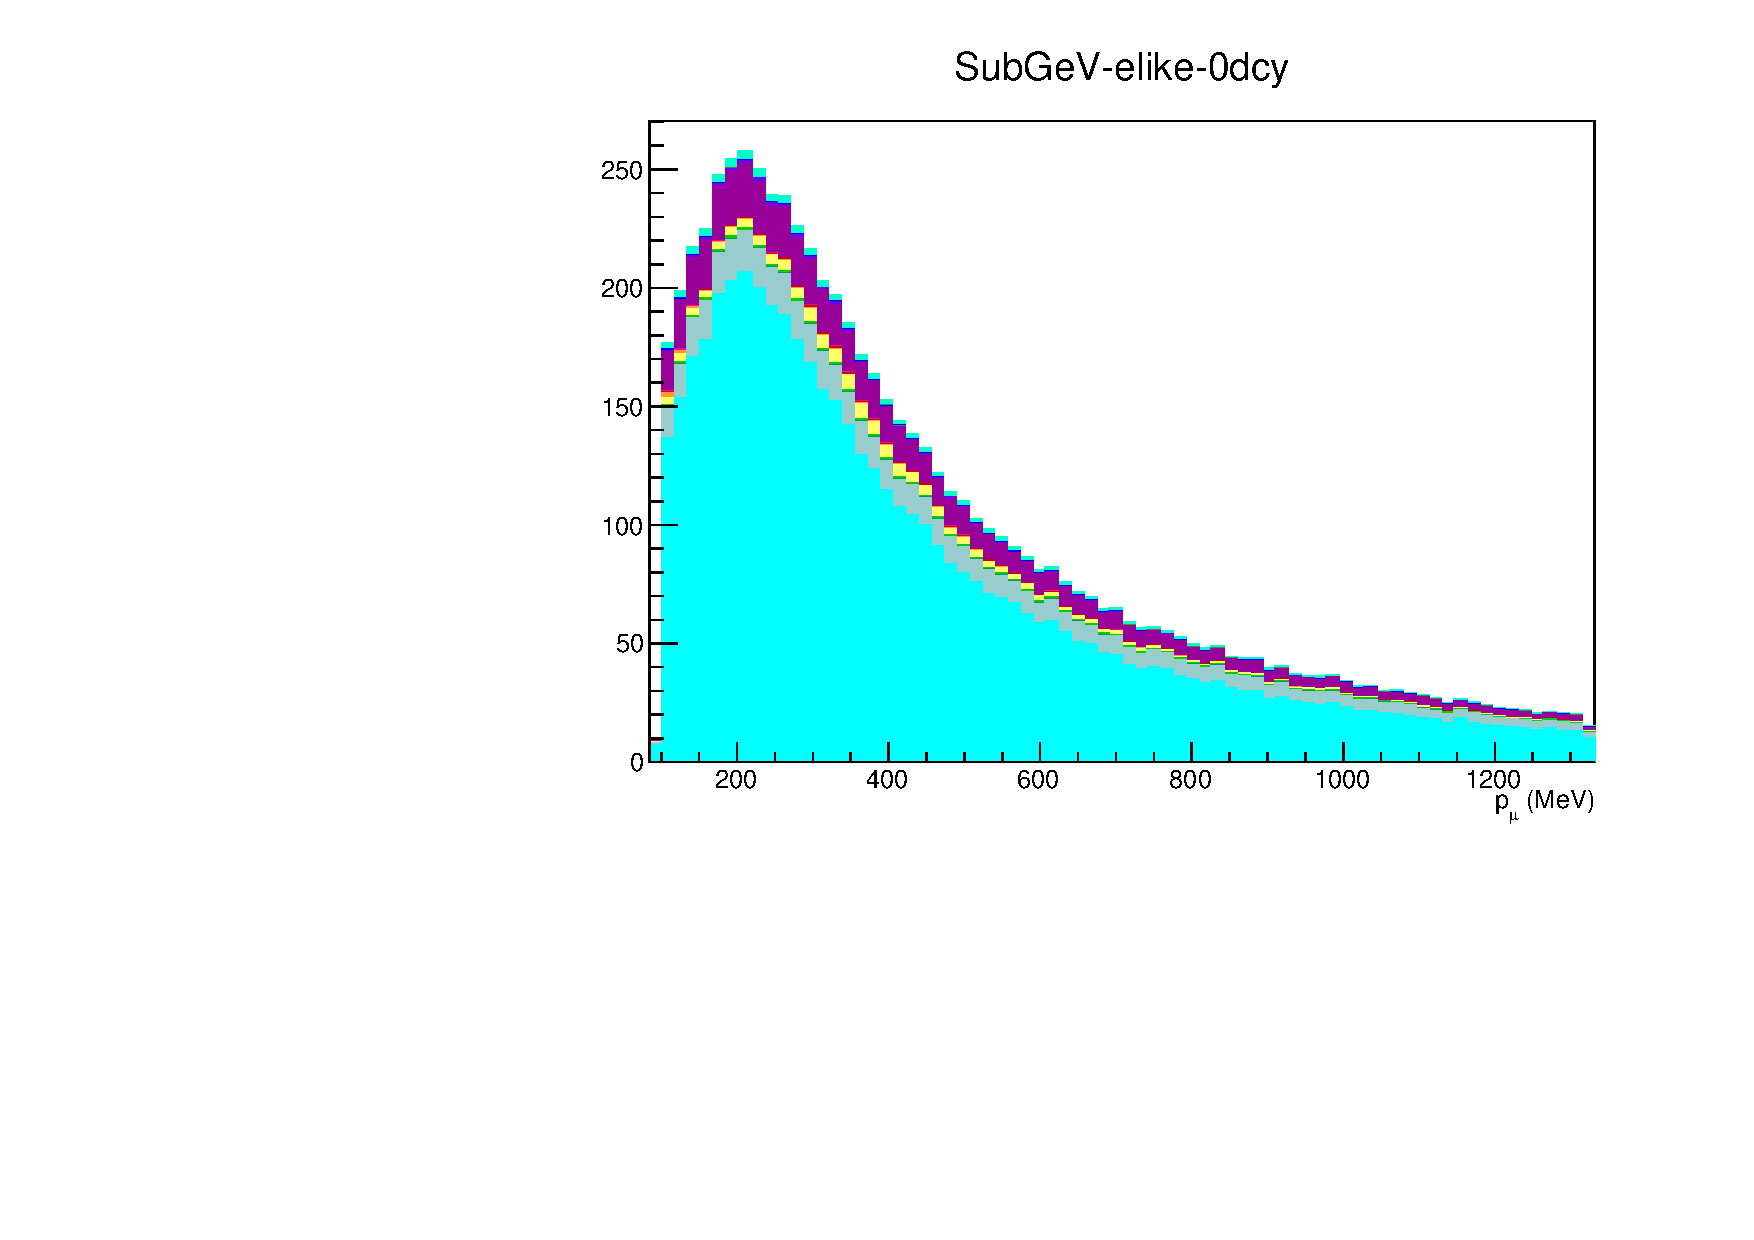
\includegraphics[width=\textwidth, trim= 0 0 0 30, clip]{Figures/Selections/AtmosphericByMode/SubGeV-elike-0dcy_LepMom.pdf}
    \caption{FC Sub-GeV 1R e-like 0 de}
    \end{subfigure}
    \begin{subfigure}[t]{0.49\textwidth}
    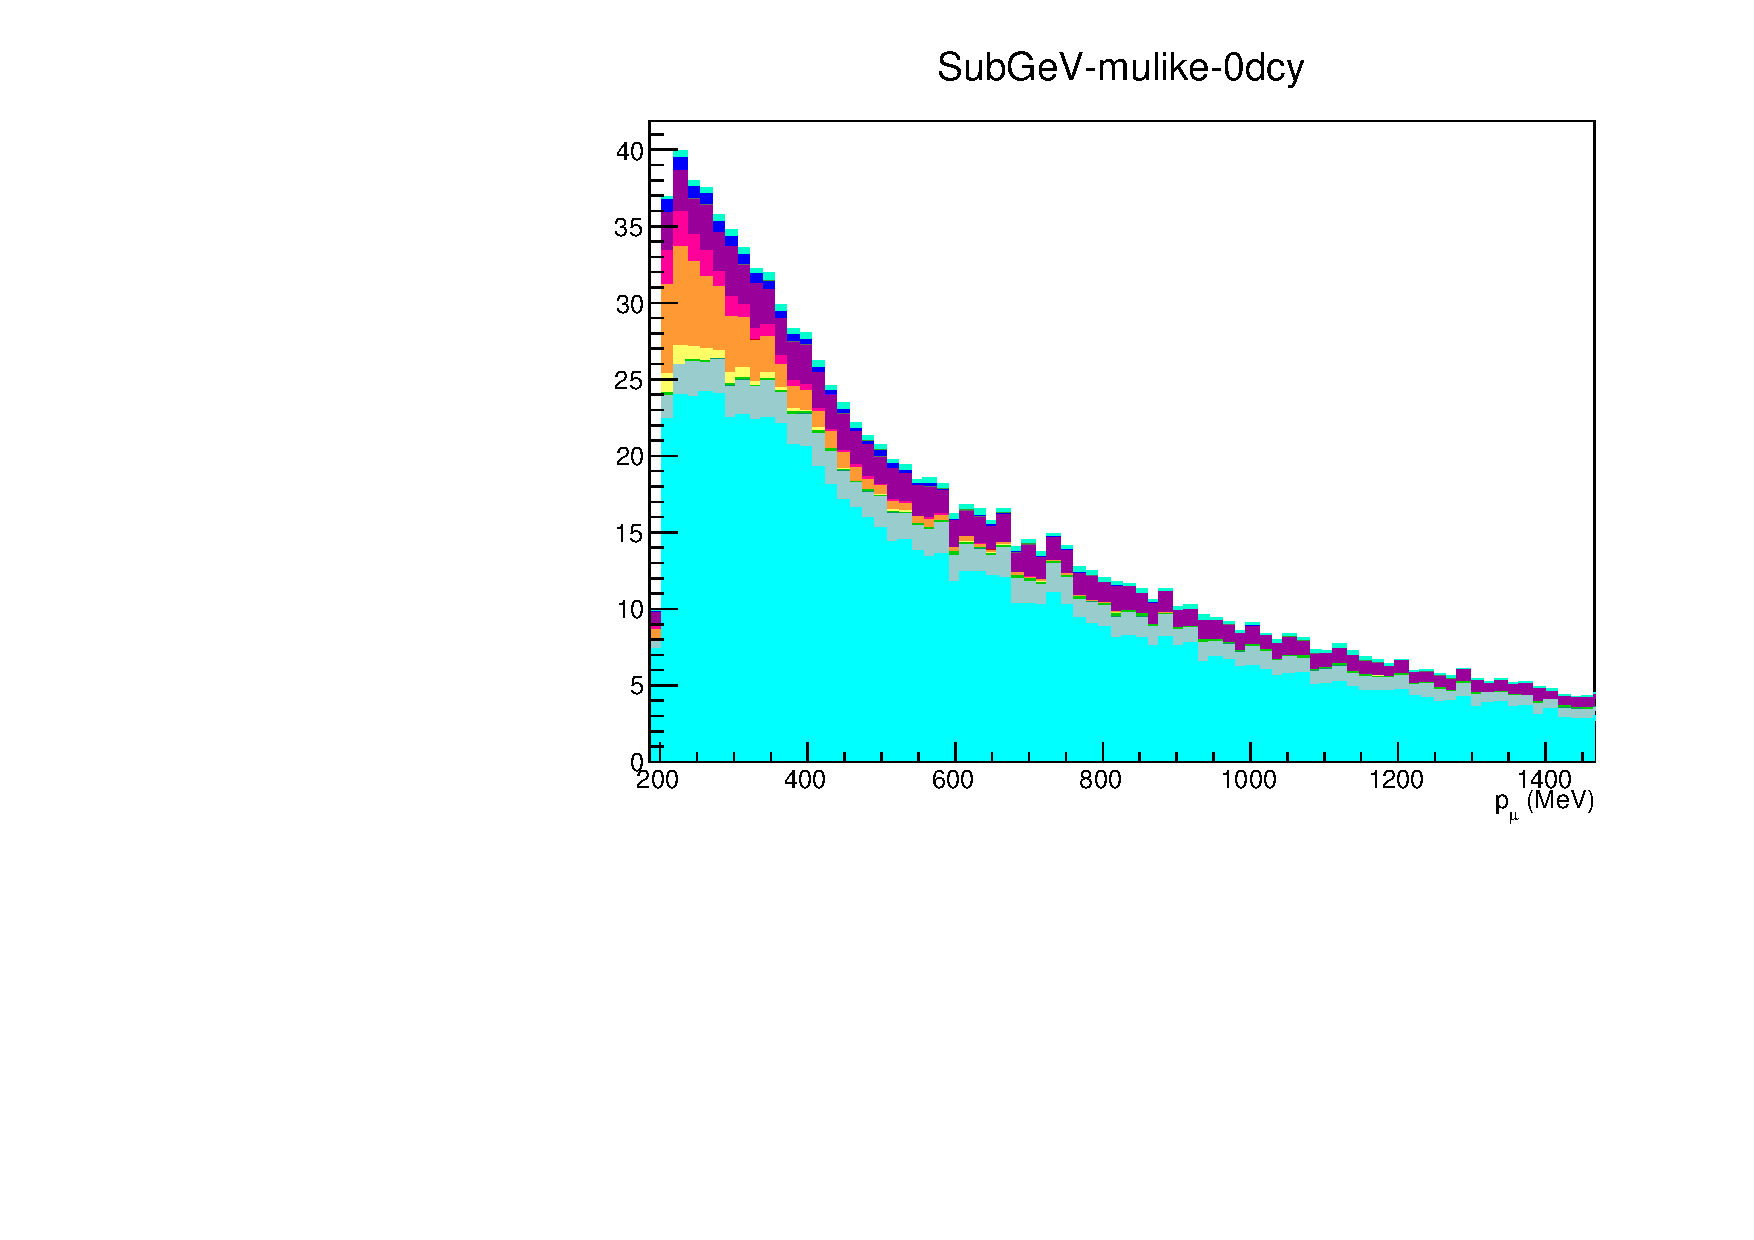
\includegraphics[width=\textwidth, trim= 0 0 0 30, clip]{Figures/Selections/AtmosphericByMode/SubGeV-mulike-0dcy_LepMom.pdf}
    \caption{FC Sub-GeV 1R $\mu$-like 0 de}
    \end{subfigure}
    \begin{subfigure}[t]{0.49\textwidth}
    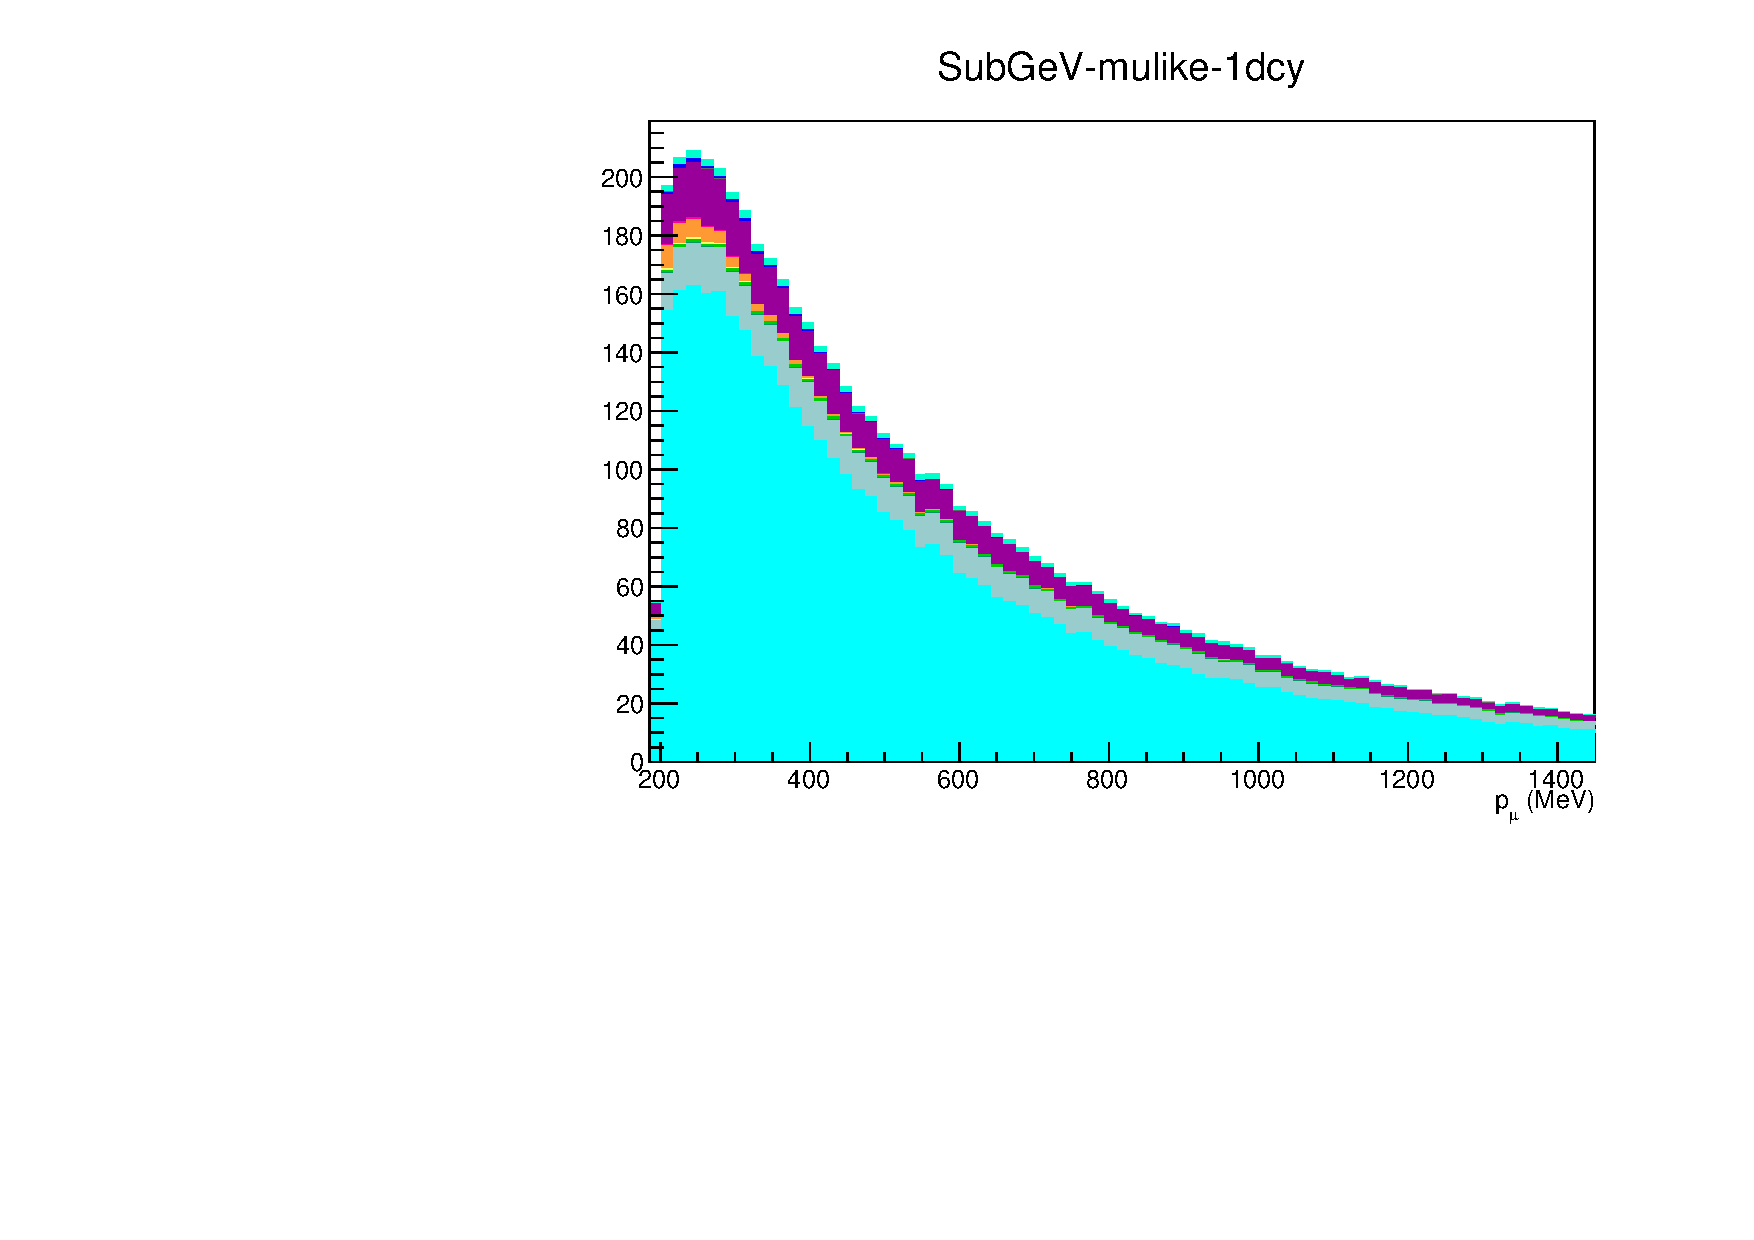
\includegraphics[width=\textwidth, trim= 0 0 0 30, clip]{Figures/Selections/AtmosphericByMode/SubGeV-mulike-1dcy_LepMom.pdf}
    \caption{FC Sub-GeV 1R $\mu$-like 1 de}
    \end{subfigure}
    \begin{subfigure}[t]{0.49\textwidth}
    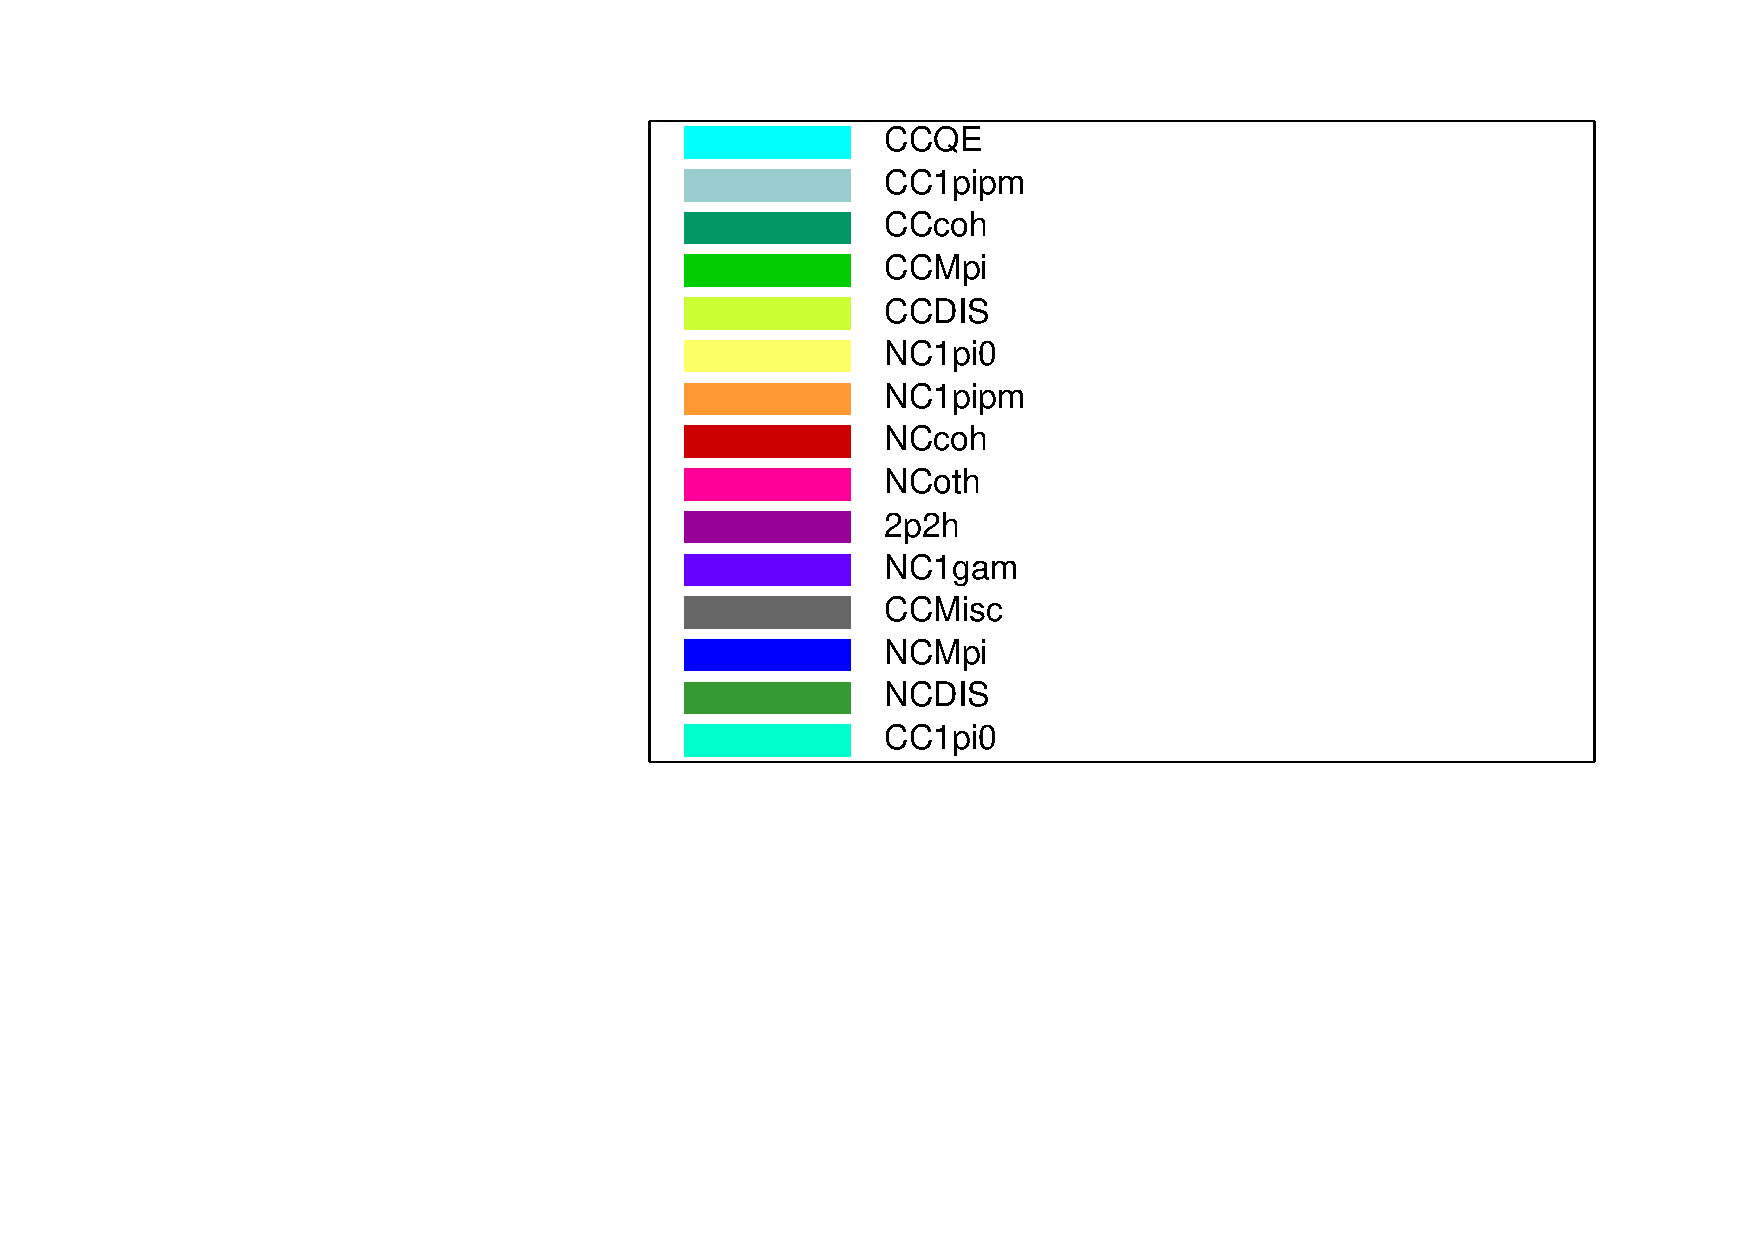
\includegraphics[page=1,width=\textwidth, trim= 0 0 0 30, clip]{Figures/Selections/AtmosphericByMode/Legend.pdf}
    \end{subfigure}
    \caption{Breakdown by interaction mode of the FC Sub-GeV atmospheric samples targeting CC0$\pi$ events.}
    \label{fig:SKSamples:FCSubGeVCC0pi}
\end{figure}

\begin{figure}[ht]
    \begin{subfigure}[t]{0.49\textwidth}
    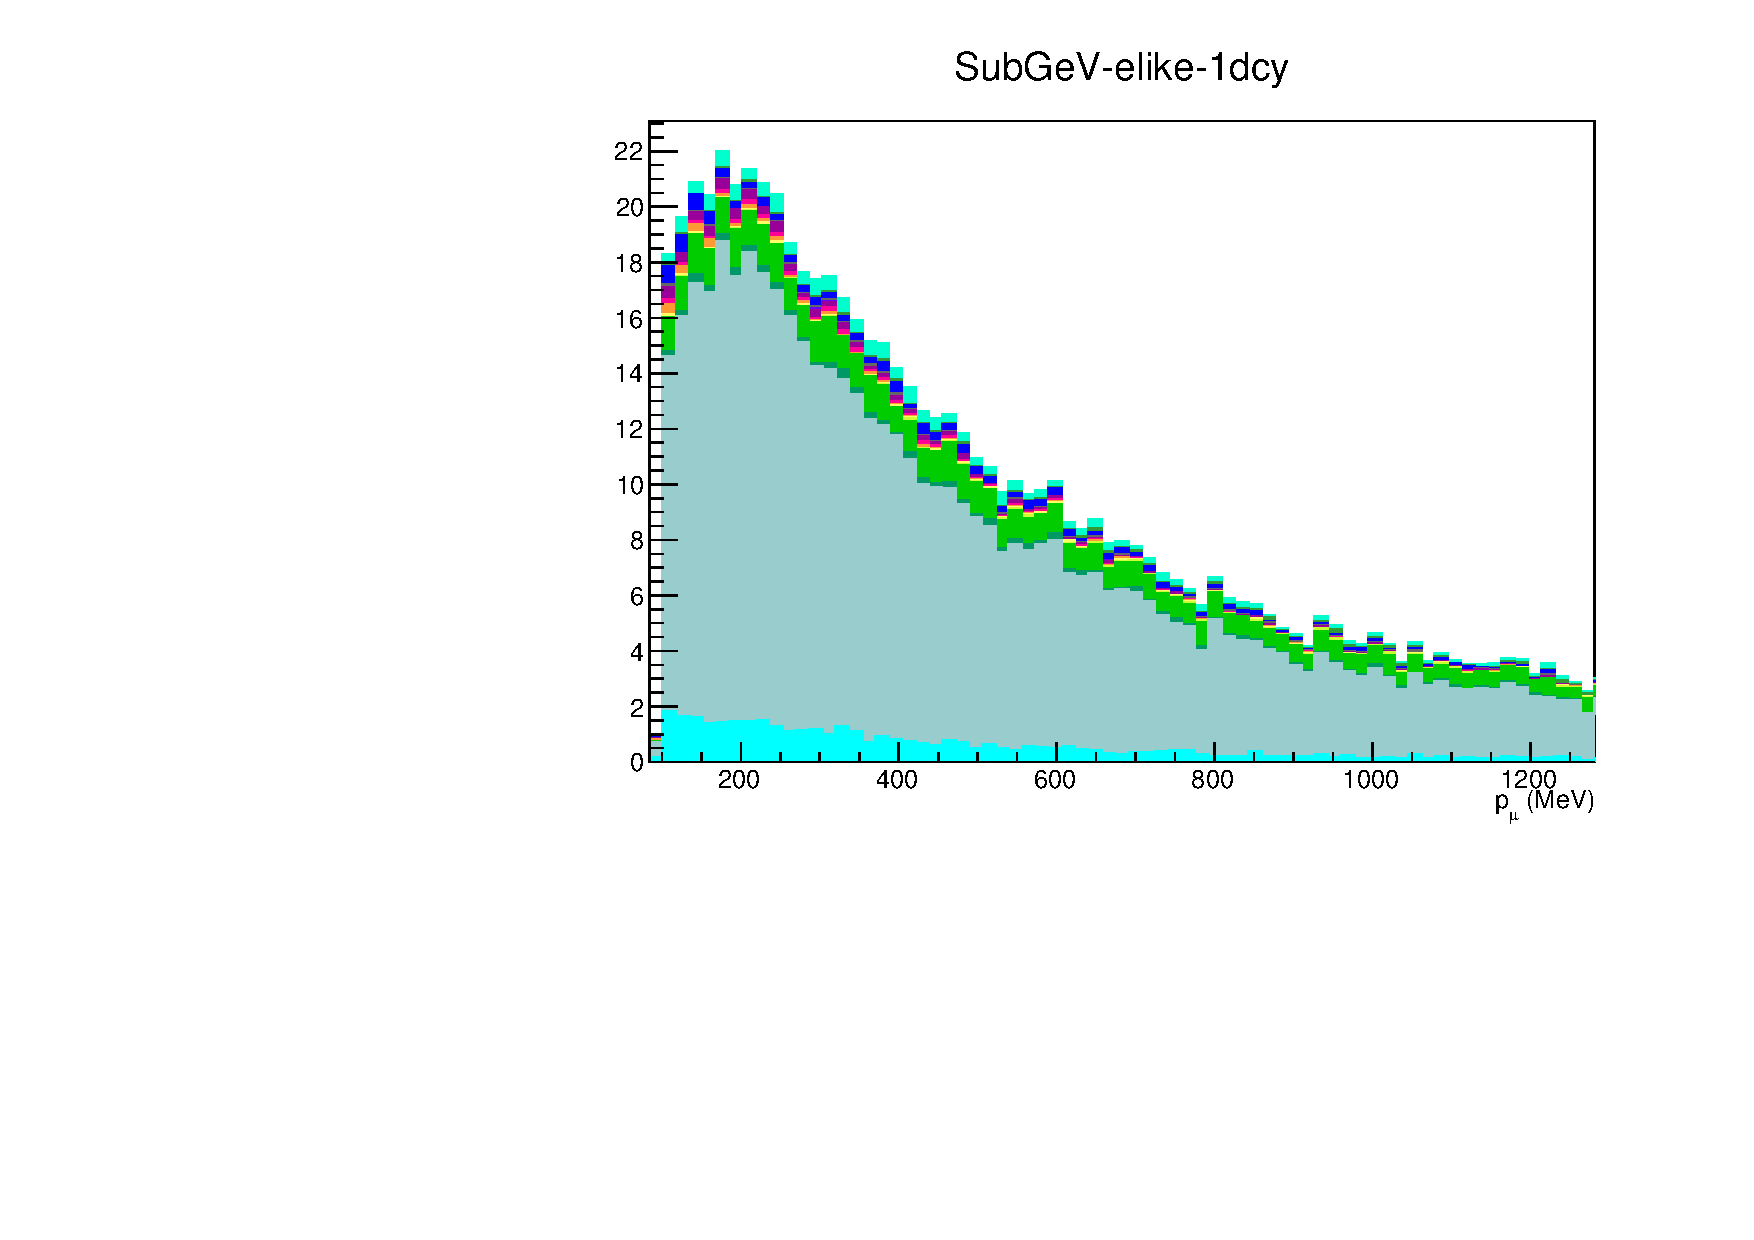
\includegraphics[width=\textwidth, trim= 0 0 0 30, clip]{Figures/Selections/AtmosphericByMode/SubGeV-elike-1dcy_LepMom.pdf}
    \caption{FC Sub-GeV 1R e-like 1 de}
    \end{subfigure}
    \begin{subfigure}[t]{0.49\textwidth}
    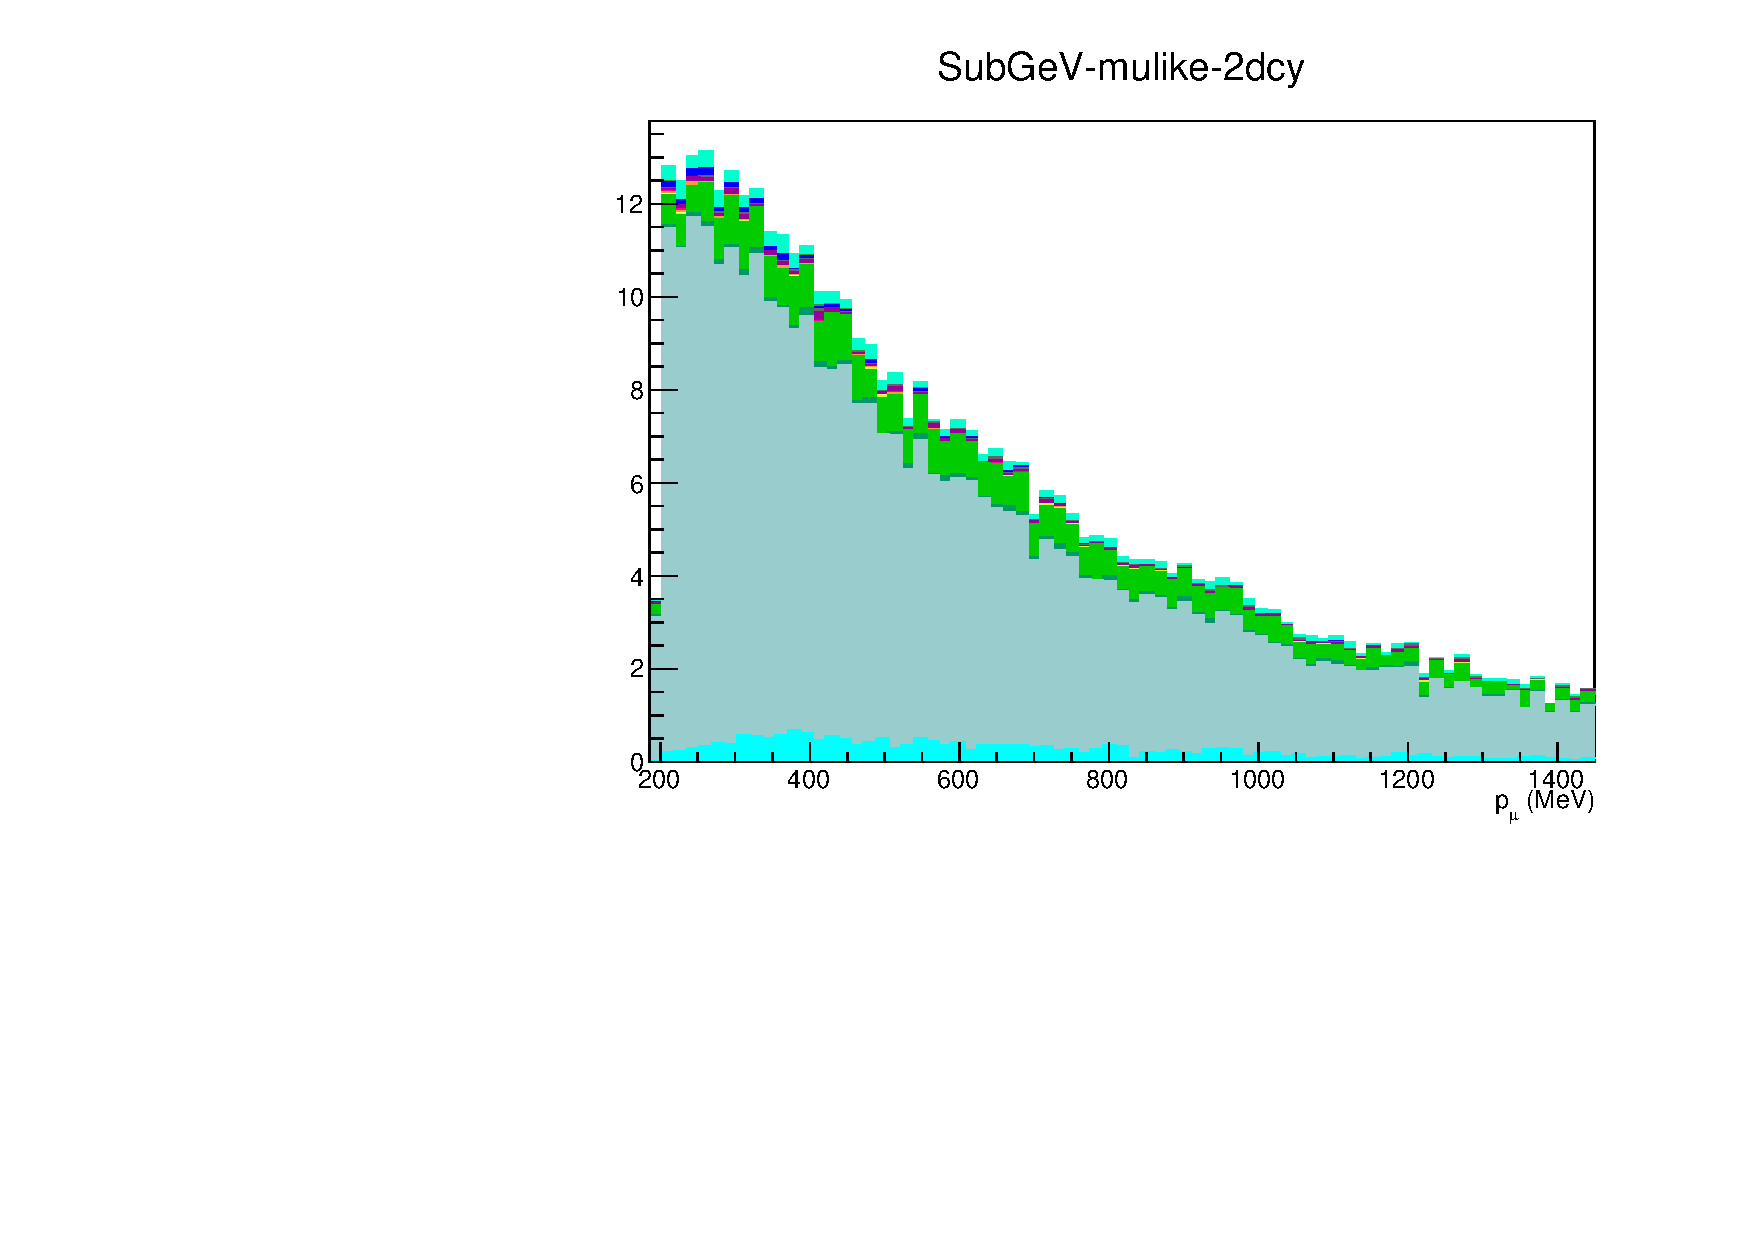
\includegraphics[width=\textwidth, trim= 0 0 0 30, clip]{Figures/Selections/AtmosphericByMode/SubGeV-mulike-2dcy_LepMom.pdf}
    \caption{FC Sub-GeV 1R $\mu$-like 2 de}
    \end{subfigure}
    \begin{subfigure}[t]{0.49\textwidth}
    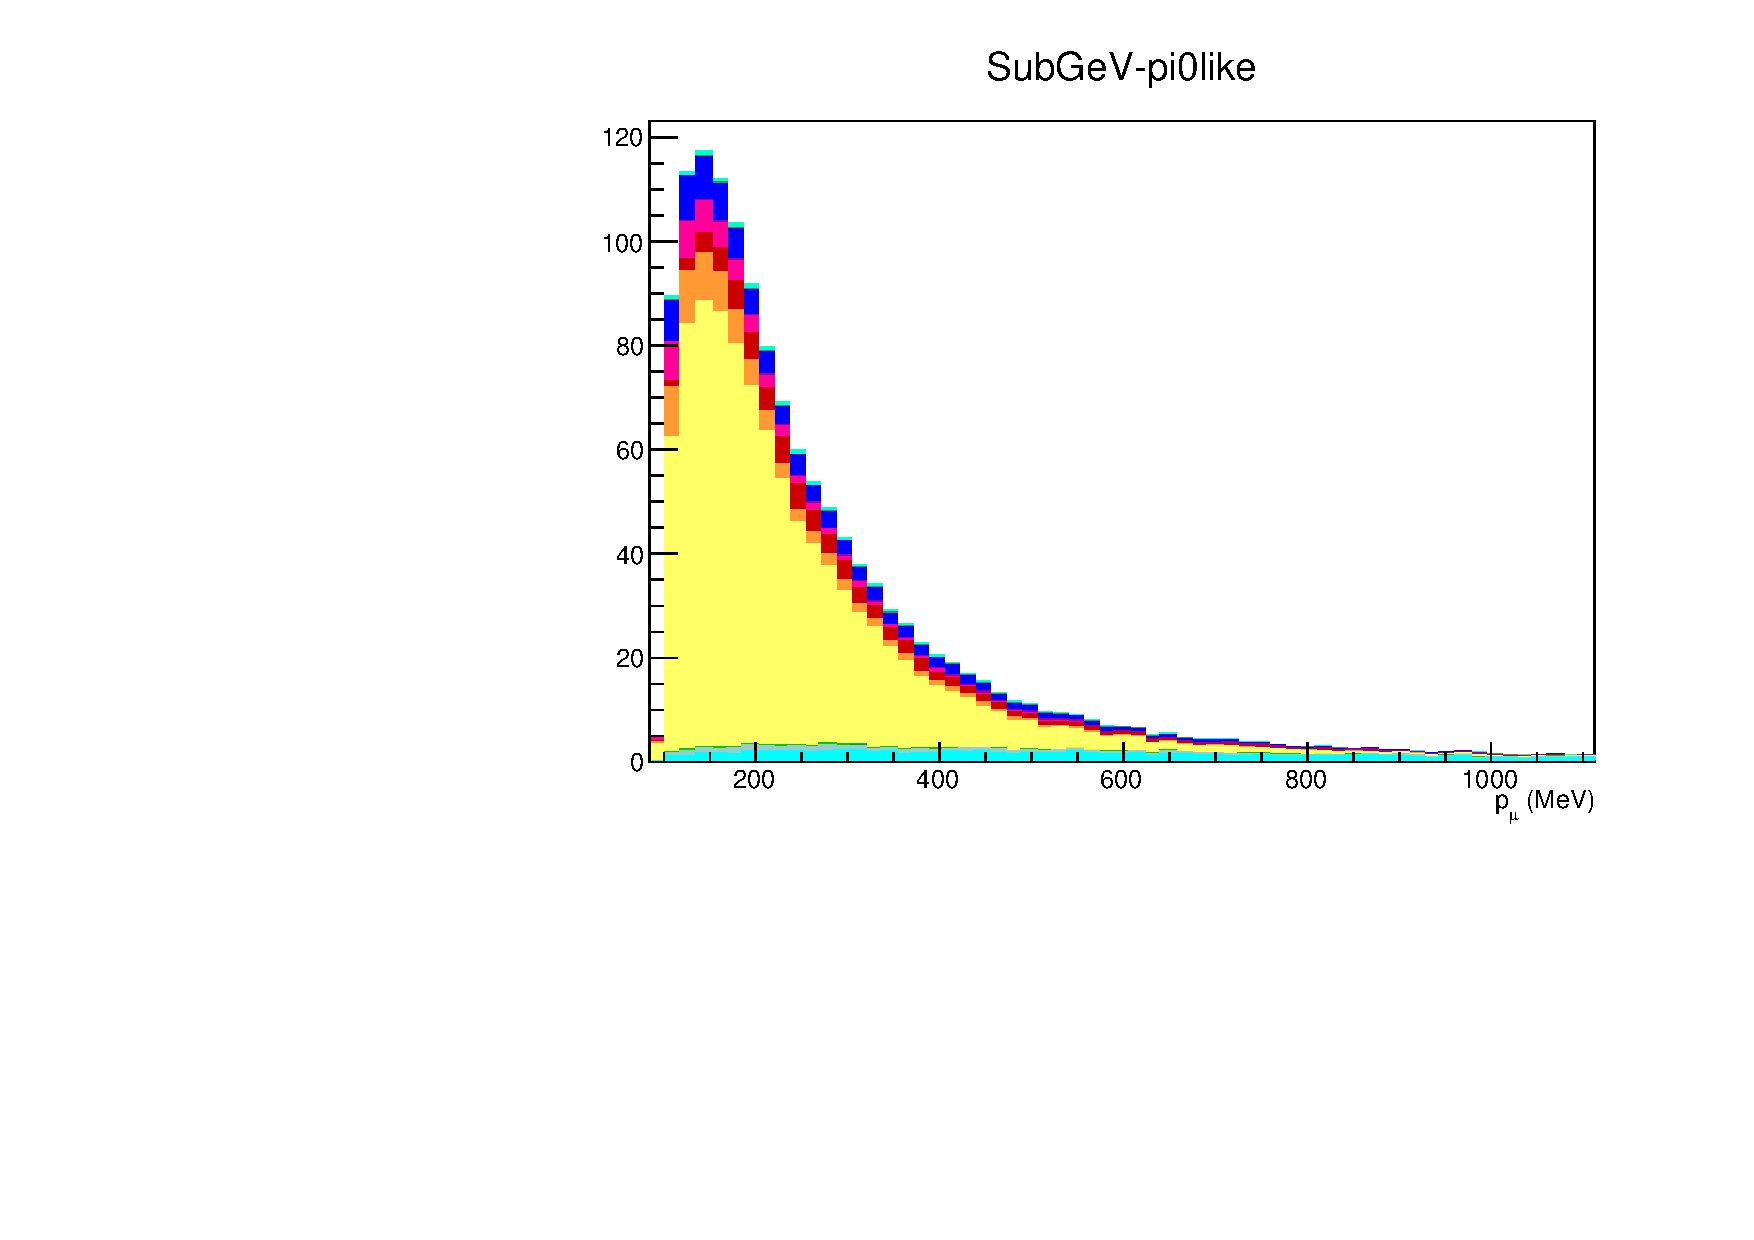
\includegraphics[width=\textwidth, trim= 0 0 0 30, clip]{Figures/Selections/AtmosphericByMode/SubGeV-pi0like_LepMom.pdf}
    \caption{FC Sub-GeV 2R $\pi^{0}$-like}
    \end{subfigure}
    \begin{subfigure}[t]{0.49\textwidth}
    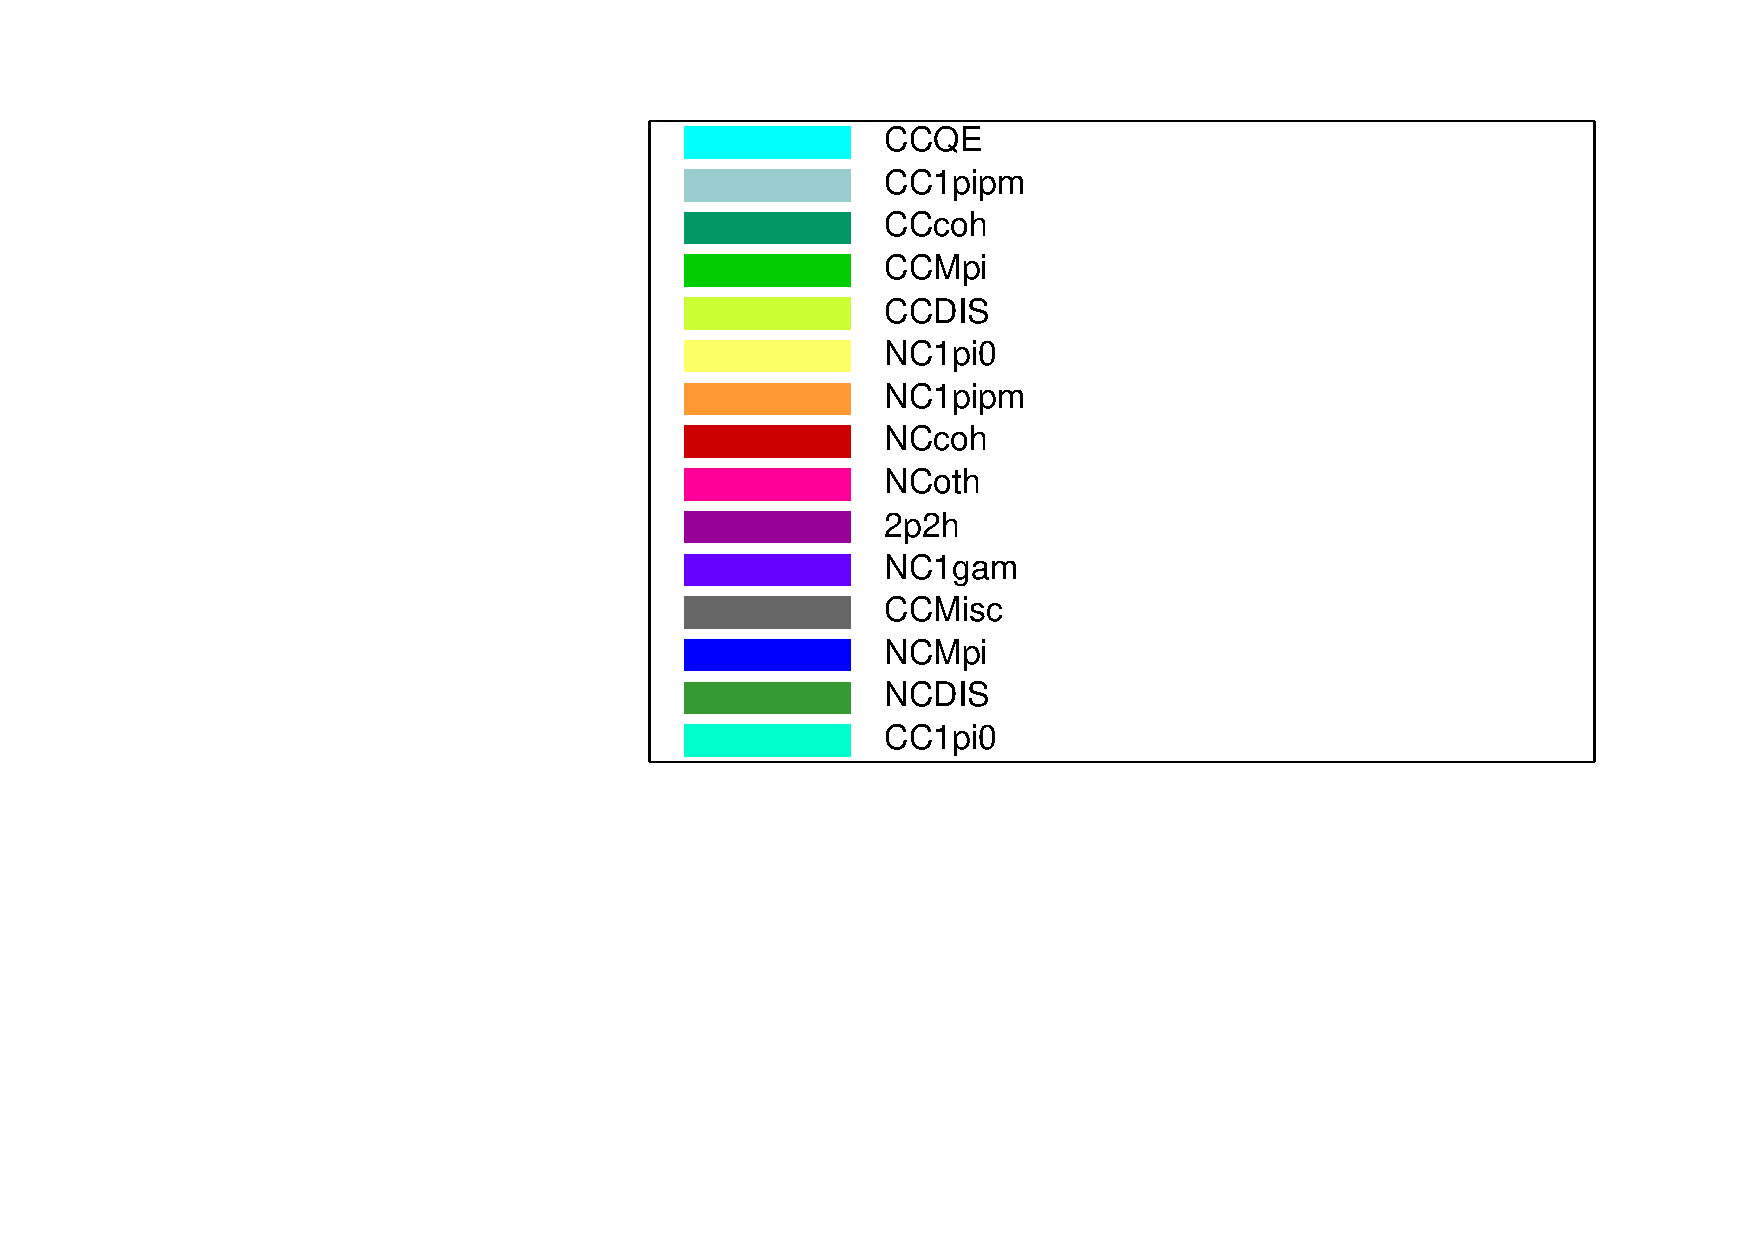
\includegraphics[page=1,width=\textwidth, trim= 0 0 0 30, clip]{Figures/Selections/AtmosphericByMode/Legend.pdf}
    \end{subfigure}
    \caption{Breakdown by interaction mode of the FC Sub-GeV atmospheric samples targeting single pion events.}
    \label{fig:SKSamples:FCSubGeVCC1pi}
\end{figure}

\clearpage
\section{Fully Contained Multi-GeV Samples}
The interaction mode breakdown of fully contained multi-GeV samples is highlighted in \autoref{fig:SKSamples:FCMultiGeV}. Due to the event selection applied in SK which targets $\pi^+$ and $\pi^-$ separation, the $\nu_e$ sample mainly consists of events with pions (single pion production or multi-pion/DIS interactions). The pion separation is explained in Section \autoref{sec:SelsAndSysts_Sels_Atms}. This reasoning also explains the significant CCQE contribution of the $\bar{\nu}_e$ sample. The muon-like sample is dominated by CCQE interactions with $\sim10-15\%$ 2p2h and CC1$\pi$ contribution of events.

\begin{figure}[ht]
    \begin{subfigure}[t]{0.49\textwidth}
    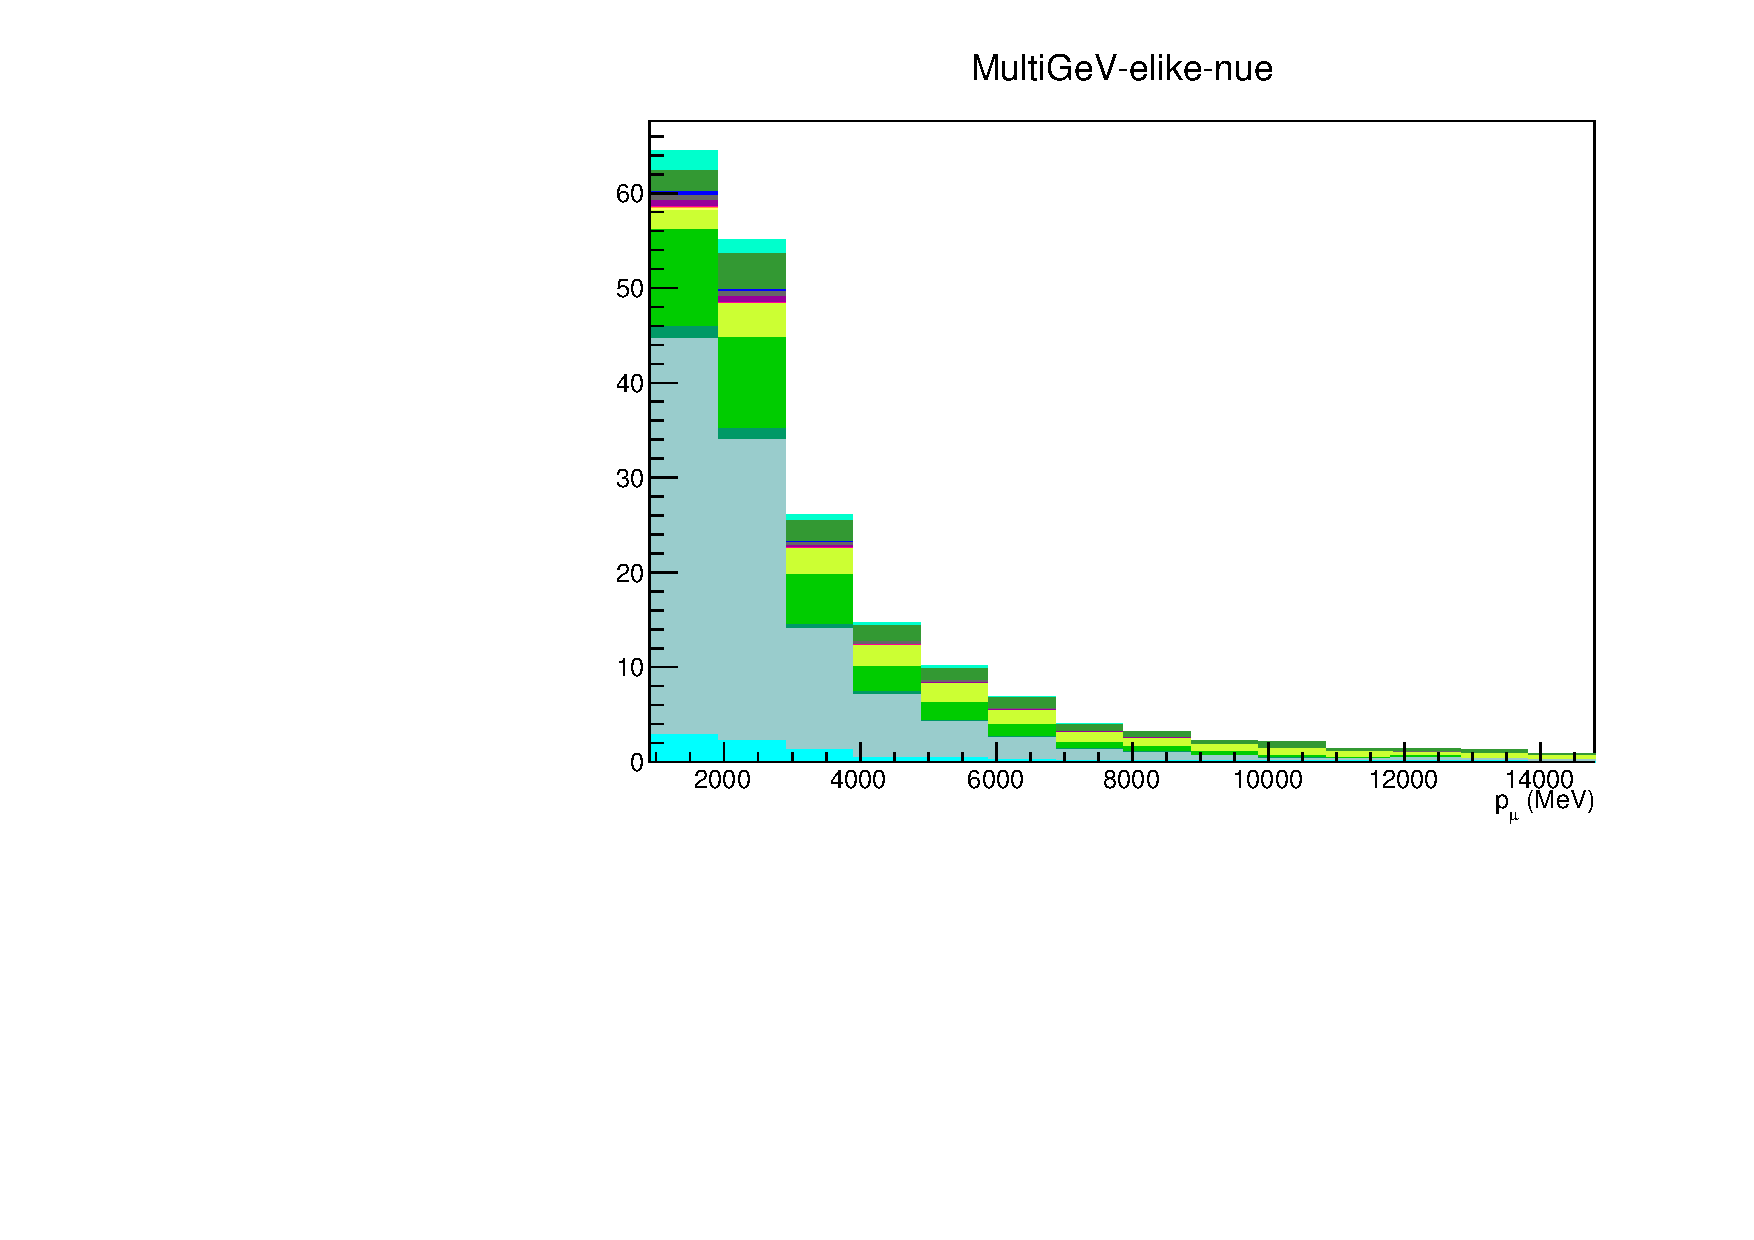
\includegraphics[width=\textwidth, trim= 0 0 0 30, clip]{Figures/Selections/AtmosphericByMode/MultiGeV-elike-nue_LepMom.pdf}
    \caption{FC Multi-GeV single ring $\nu_e$-like}
    \end{subfigure}
    \begin{subfigure}[t]{0.49\textwidth}
    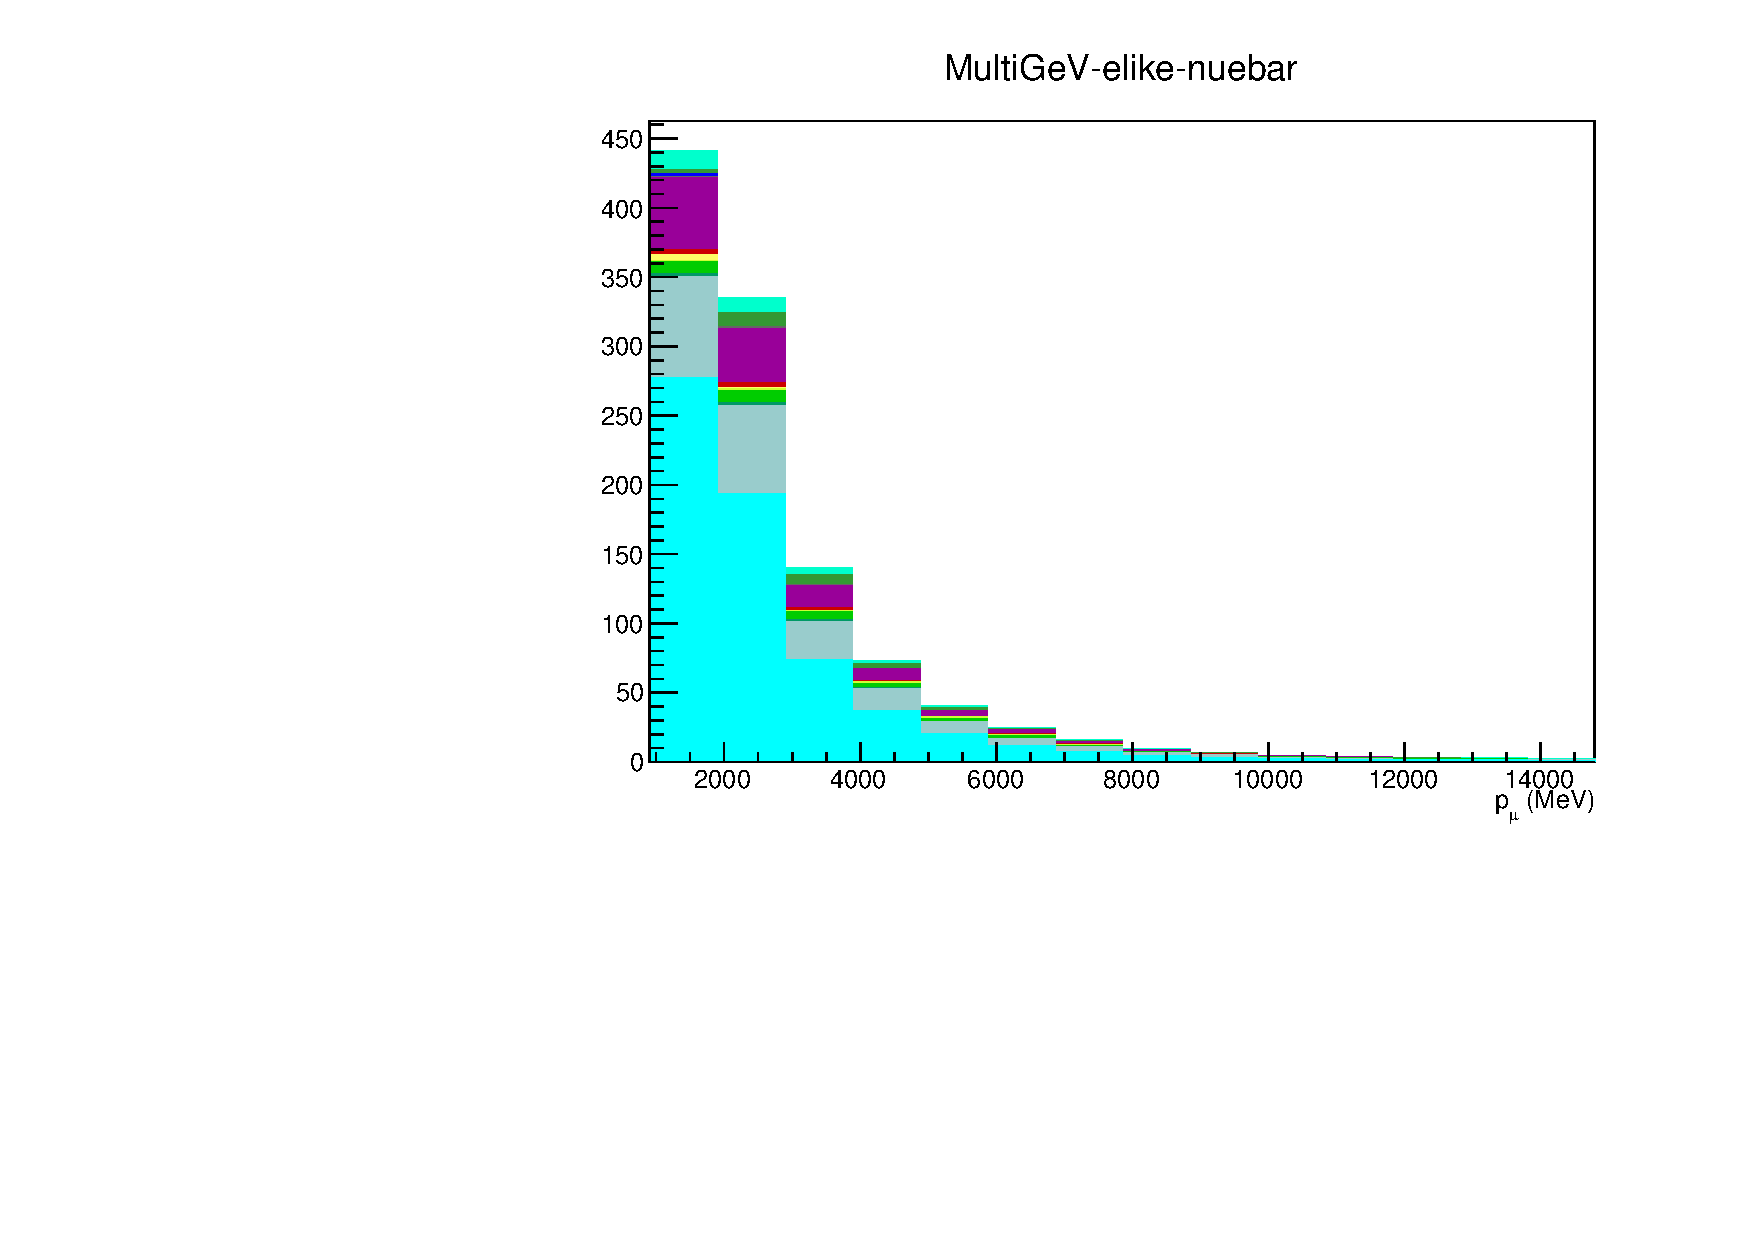
\includegraphics[width=\textwidth, trim= 0 0 0 30, clip]{Figures/Selections/AtmosphericByMode/MultiGeV-elike-nuebar_LepMom.pdf}
    \caption{FC Multi-GeV single ring $\bar{\nu}_e$-like}
    \end{subfigure}
    \begin{subfigure}[t]{0.49\textwidth}
    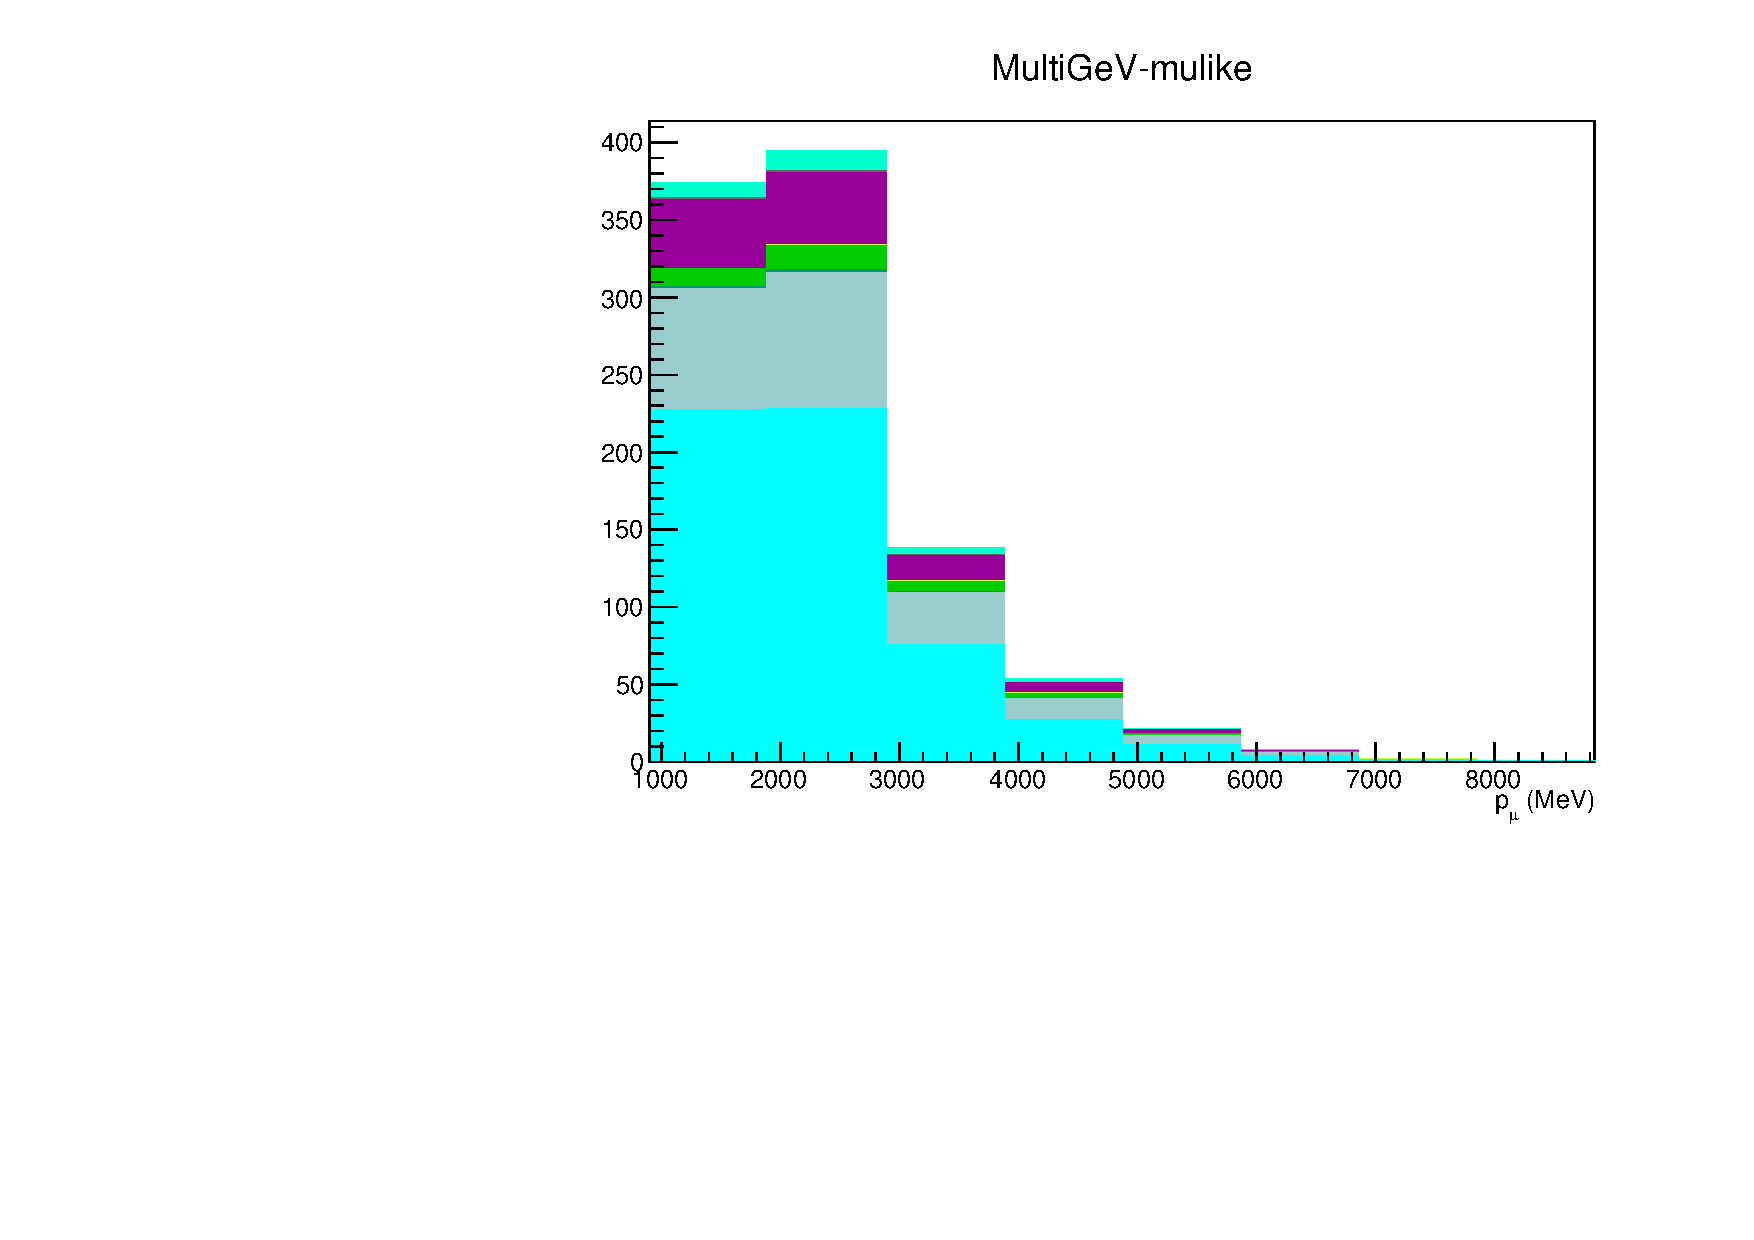
\includegraphics[width=\textwidth, trim= 0 0 0 30, clip]{Figures/Selections/AtmosphericByMode/MultiGeV-mulike_LepMom.pdf}
    \caption{FC Multi-GeV single ring $\mu$-like}
    \end{subfigure}
    \begin{subfigure}[t]{0.49\textwidth}
    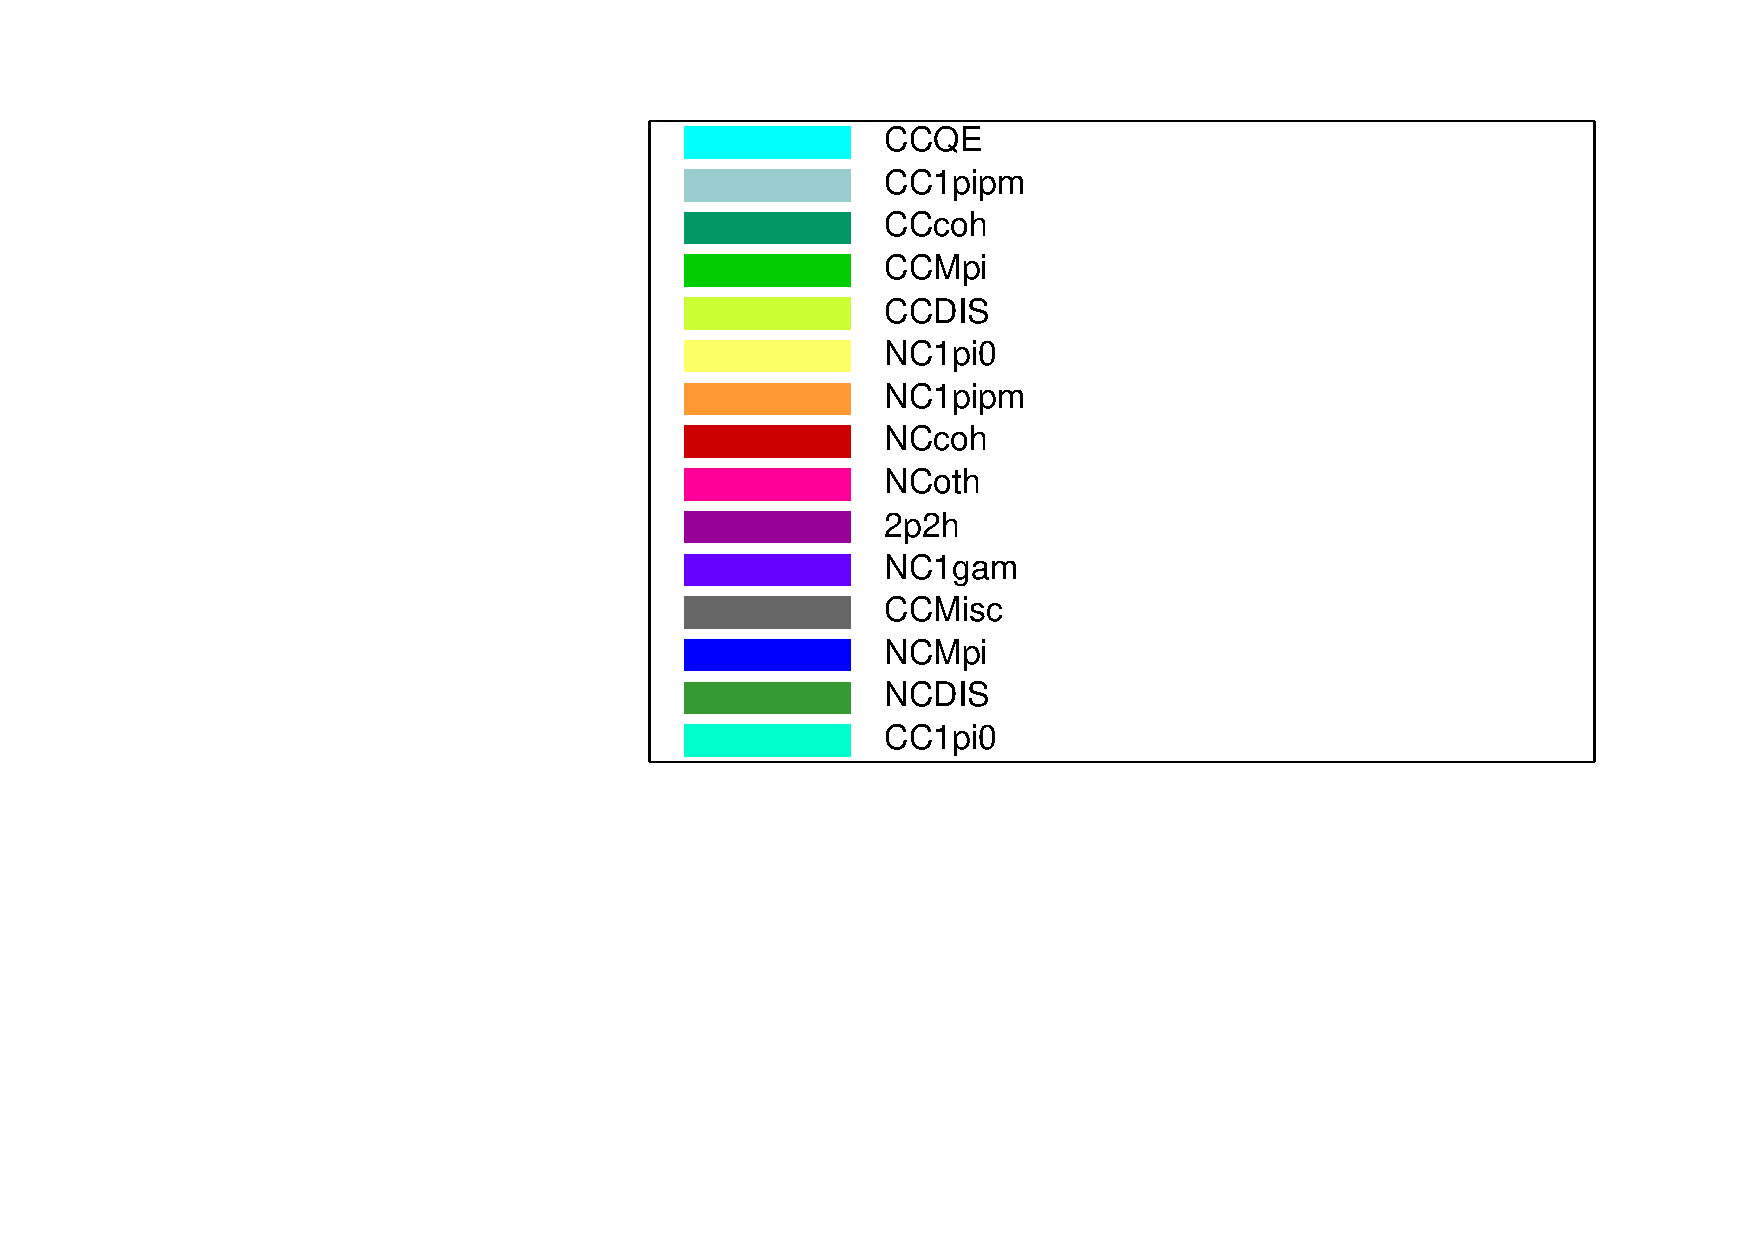
\includegraphics[page=1,width=\textwidth, trim= 0 0 0 30, clip]{Figures/Selections/AtmosphericByMode/Legend.pdf}
    \end{subfigure}

    \caption{Breakdown by interaction mode of the FC Multi-GeV single ring atmospheric samples.}
    \label{fig:SKSamples:FCMultiGeV}
\end{figure}

\clearpage
\section{Fully Contained Multi-Ring Samples}

The interaction mode breakdown of fully contained multi-ring events is shown in \autoref{fig:SKSamples:FCMultiRing}. These samples see more interaction modes contributing in general, and there is a much larger contribution from multi-pion and DIS interaction modes, compared to the other samples.

\begin{figure}[ht]
    \begin{subfigure}[t]{0.49\textwidth}
    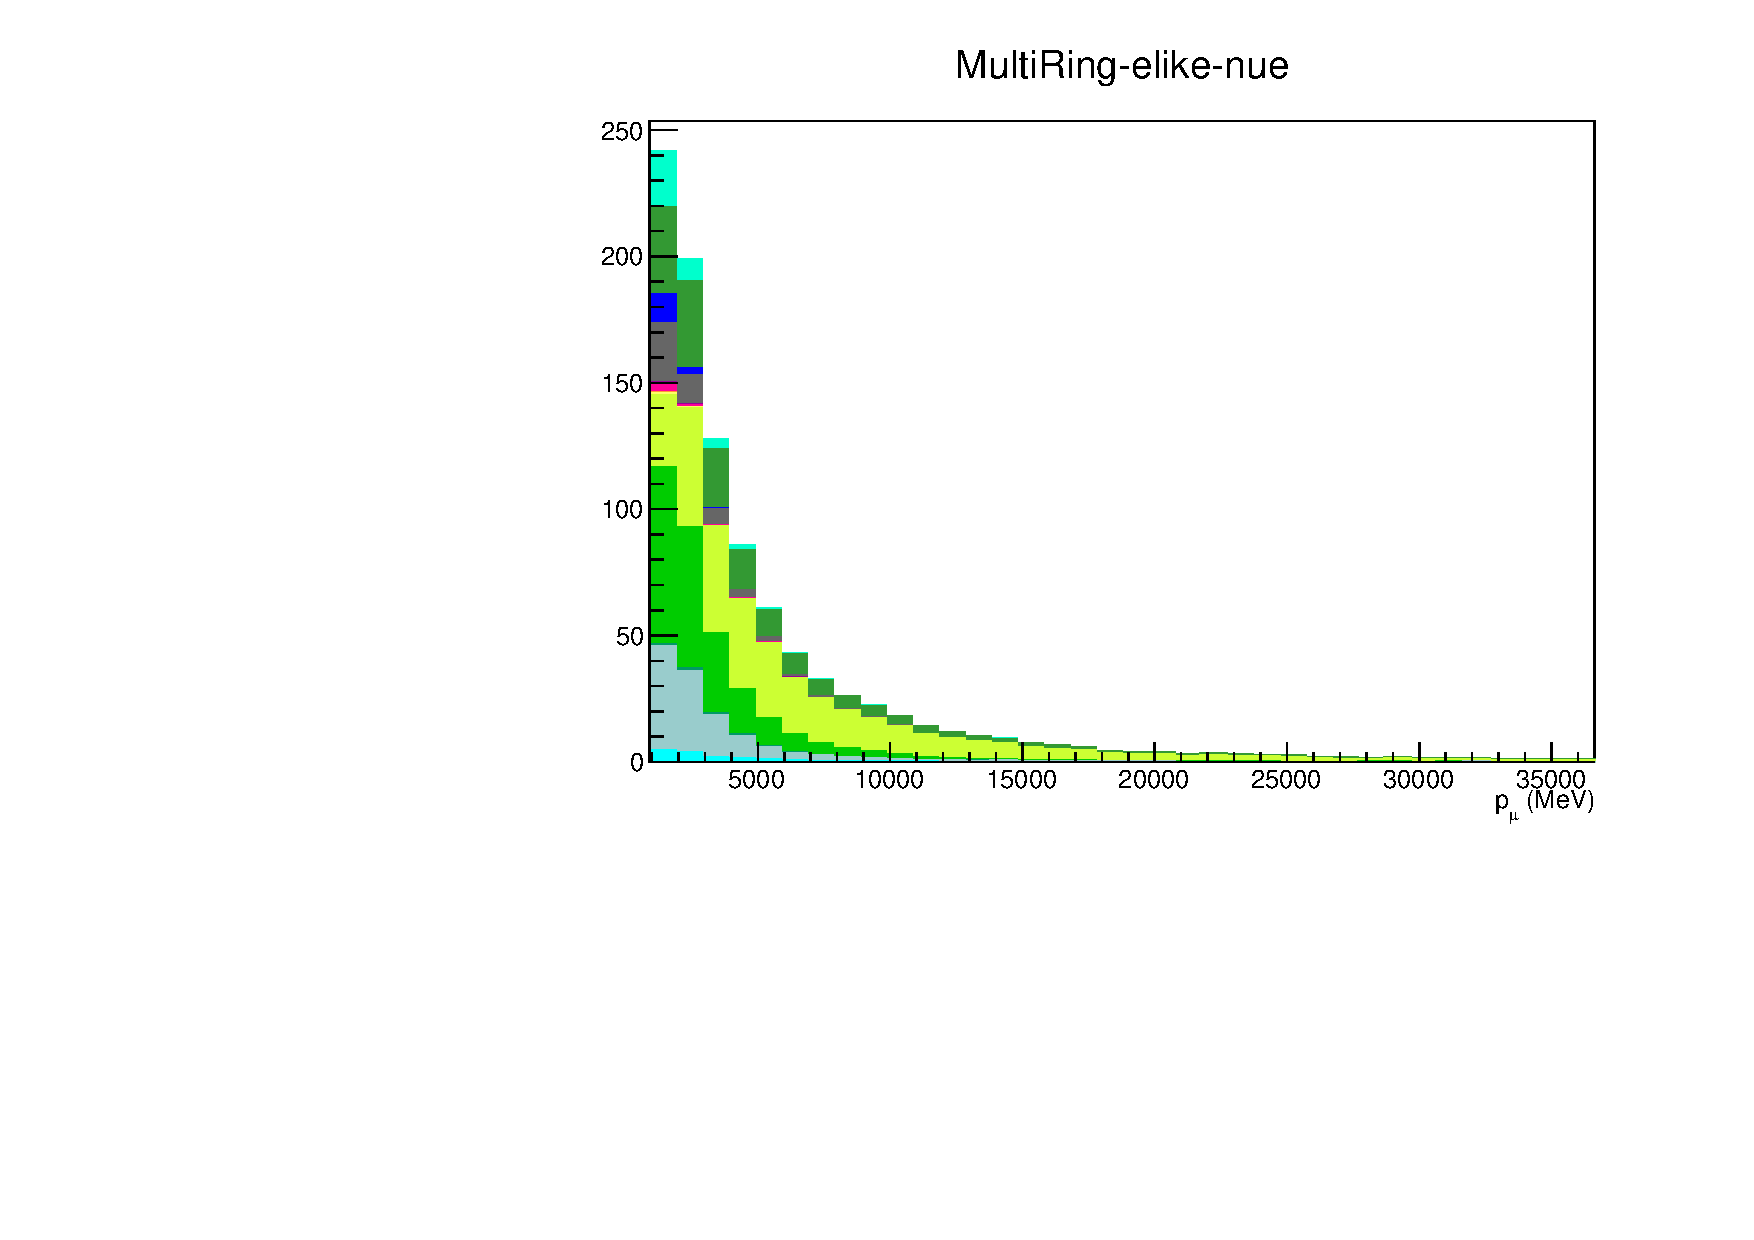
\includegraphics[width=\textwidth, trim= 0 0 0 30, clip]{Figures/Selections/AtmosphericByMode/MultiRing-elike-nue_LepMom.pdf}
    \caption{FC Multi-GeV multi-ring $\nu_e$-like}
    \end{subfigure}
    \begin{subfigure}[t]{0.49\textwidth}
    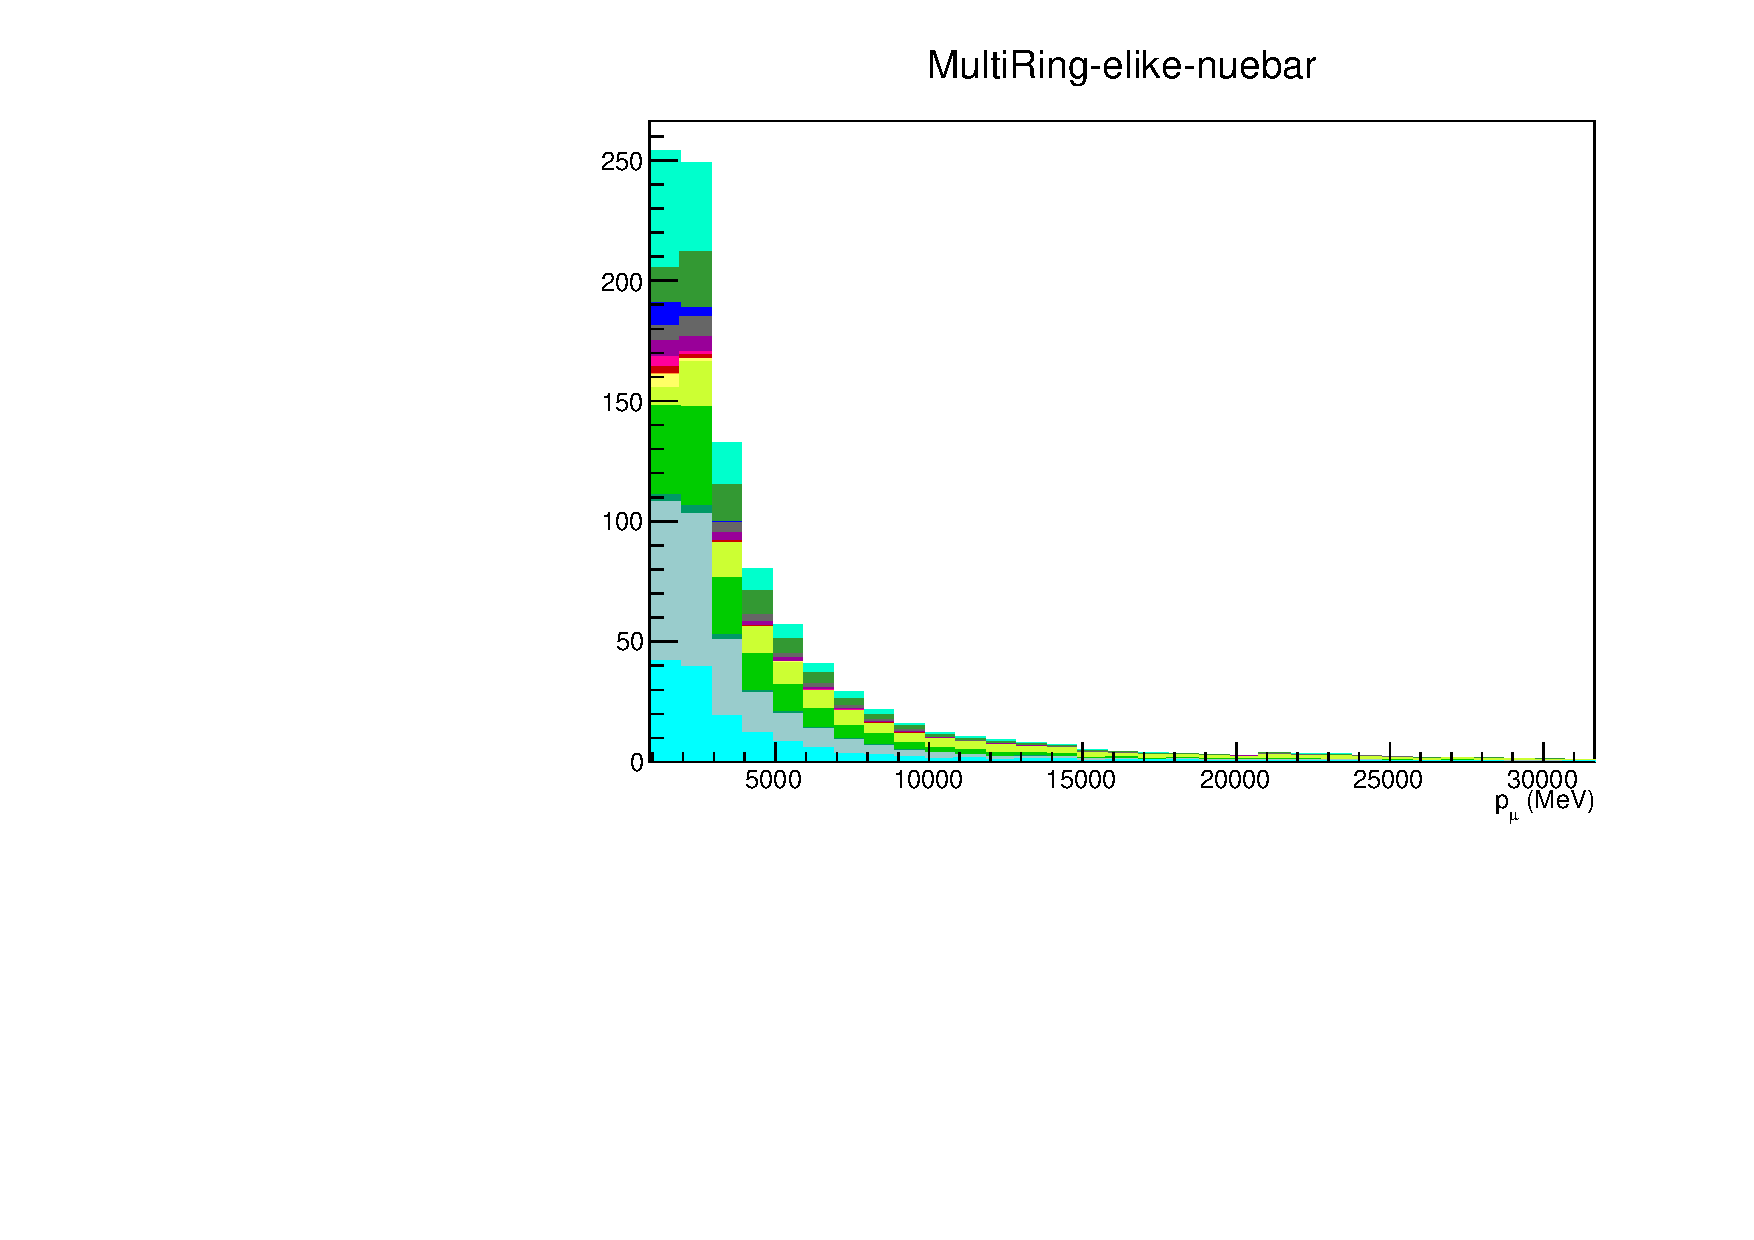
\includegraphics[width=\textwidth, trim= 0 0 0 30, clip]{Figures/Selections/AtmosphericByMode/MultiRing-elike-nuebar_LepMom.pdf}
    \caption{FC Multi-GeV multi-ring $\bar{\nu}_e$-like}
    \end{subfigure}
    \begin{subfigure}[t]{0.49\textwidth}
    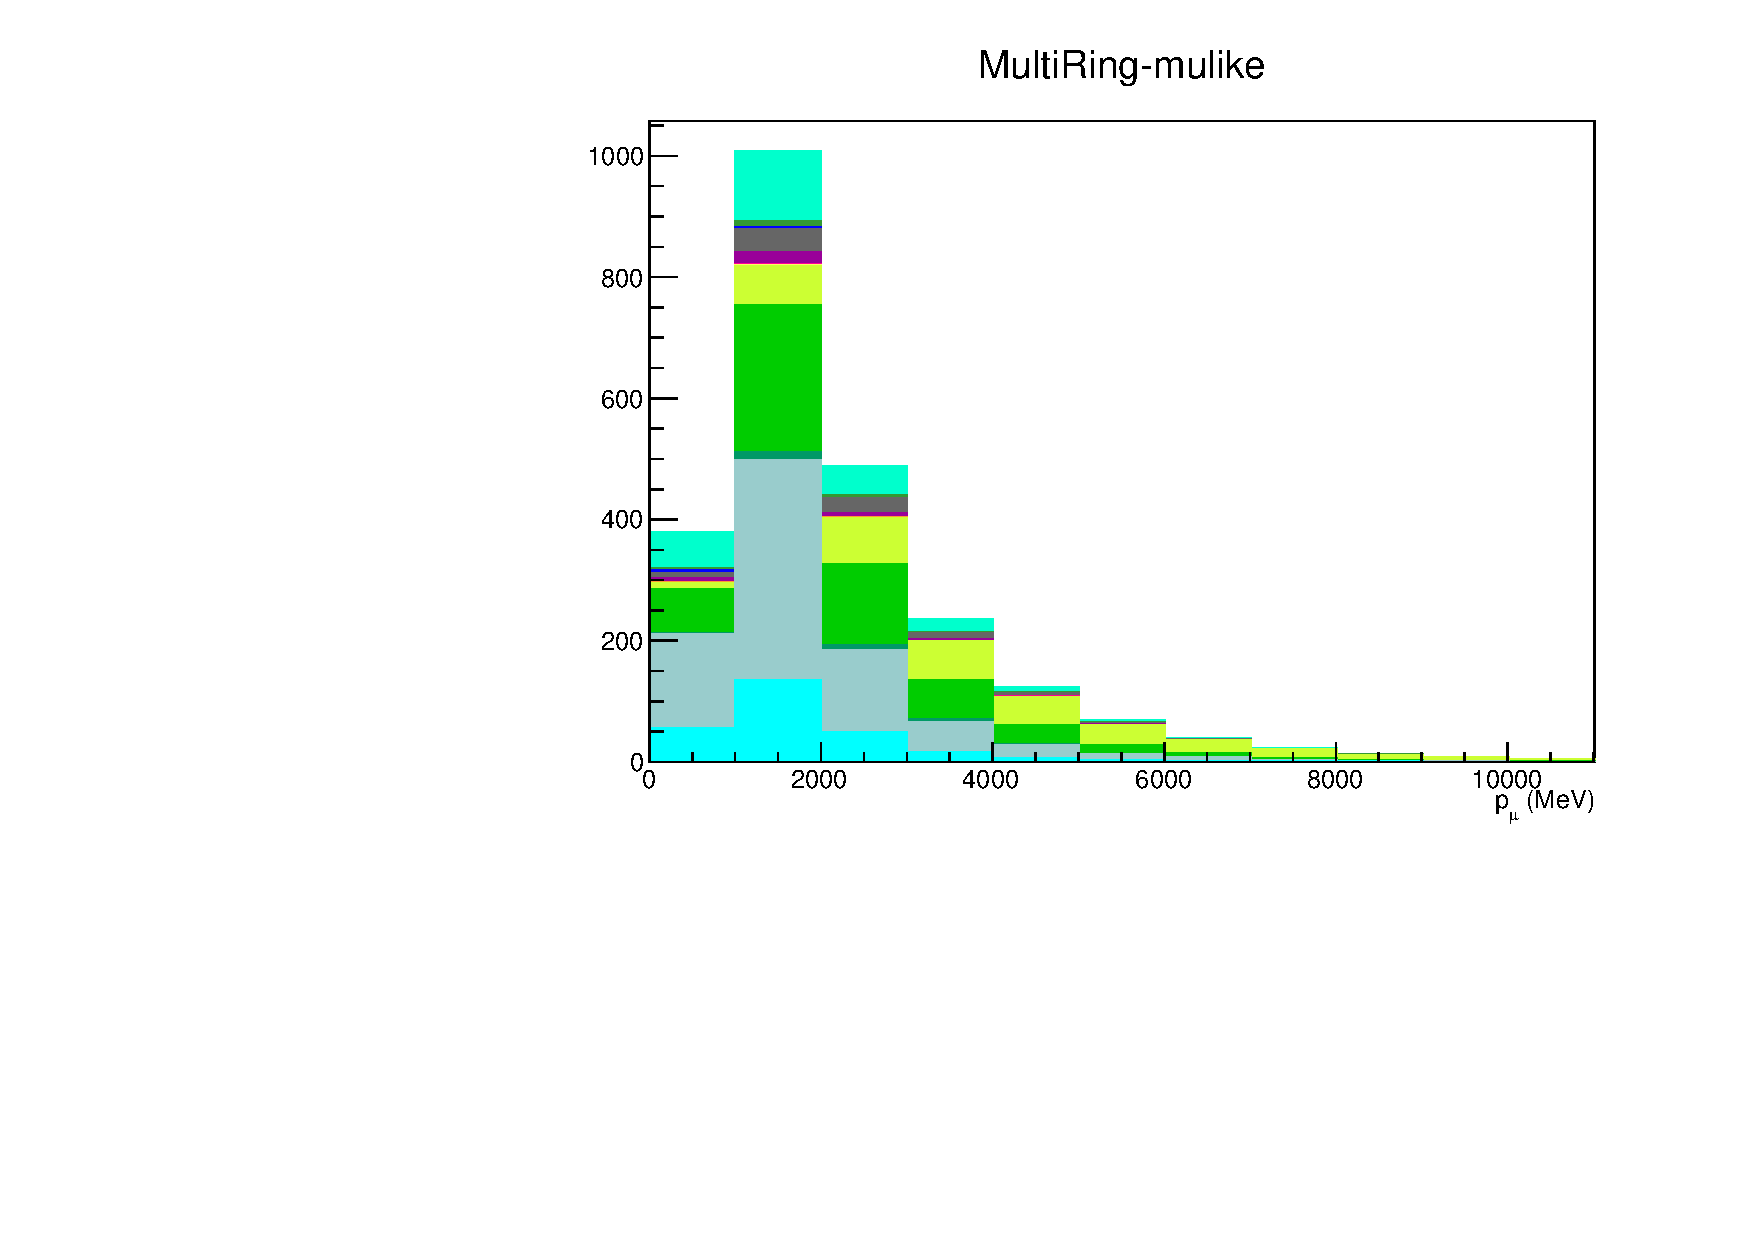
\includegraphics[width=\textwidth, trim= 0 0 0 30, clip]{Figures/Selections/AtmosphericByMode/MultiRing-mulike_LepMom.pdf}
    \caption{FC Multi-GeV multi-ring $\mu$-like}
    \end{subfigure}
    \begin{subfigure}[t]{0.49\textwidth}
    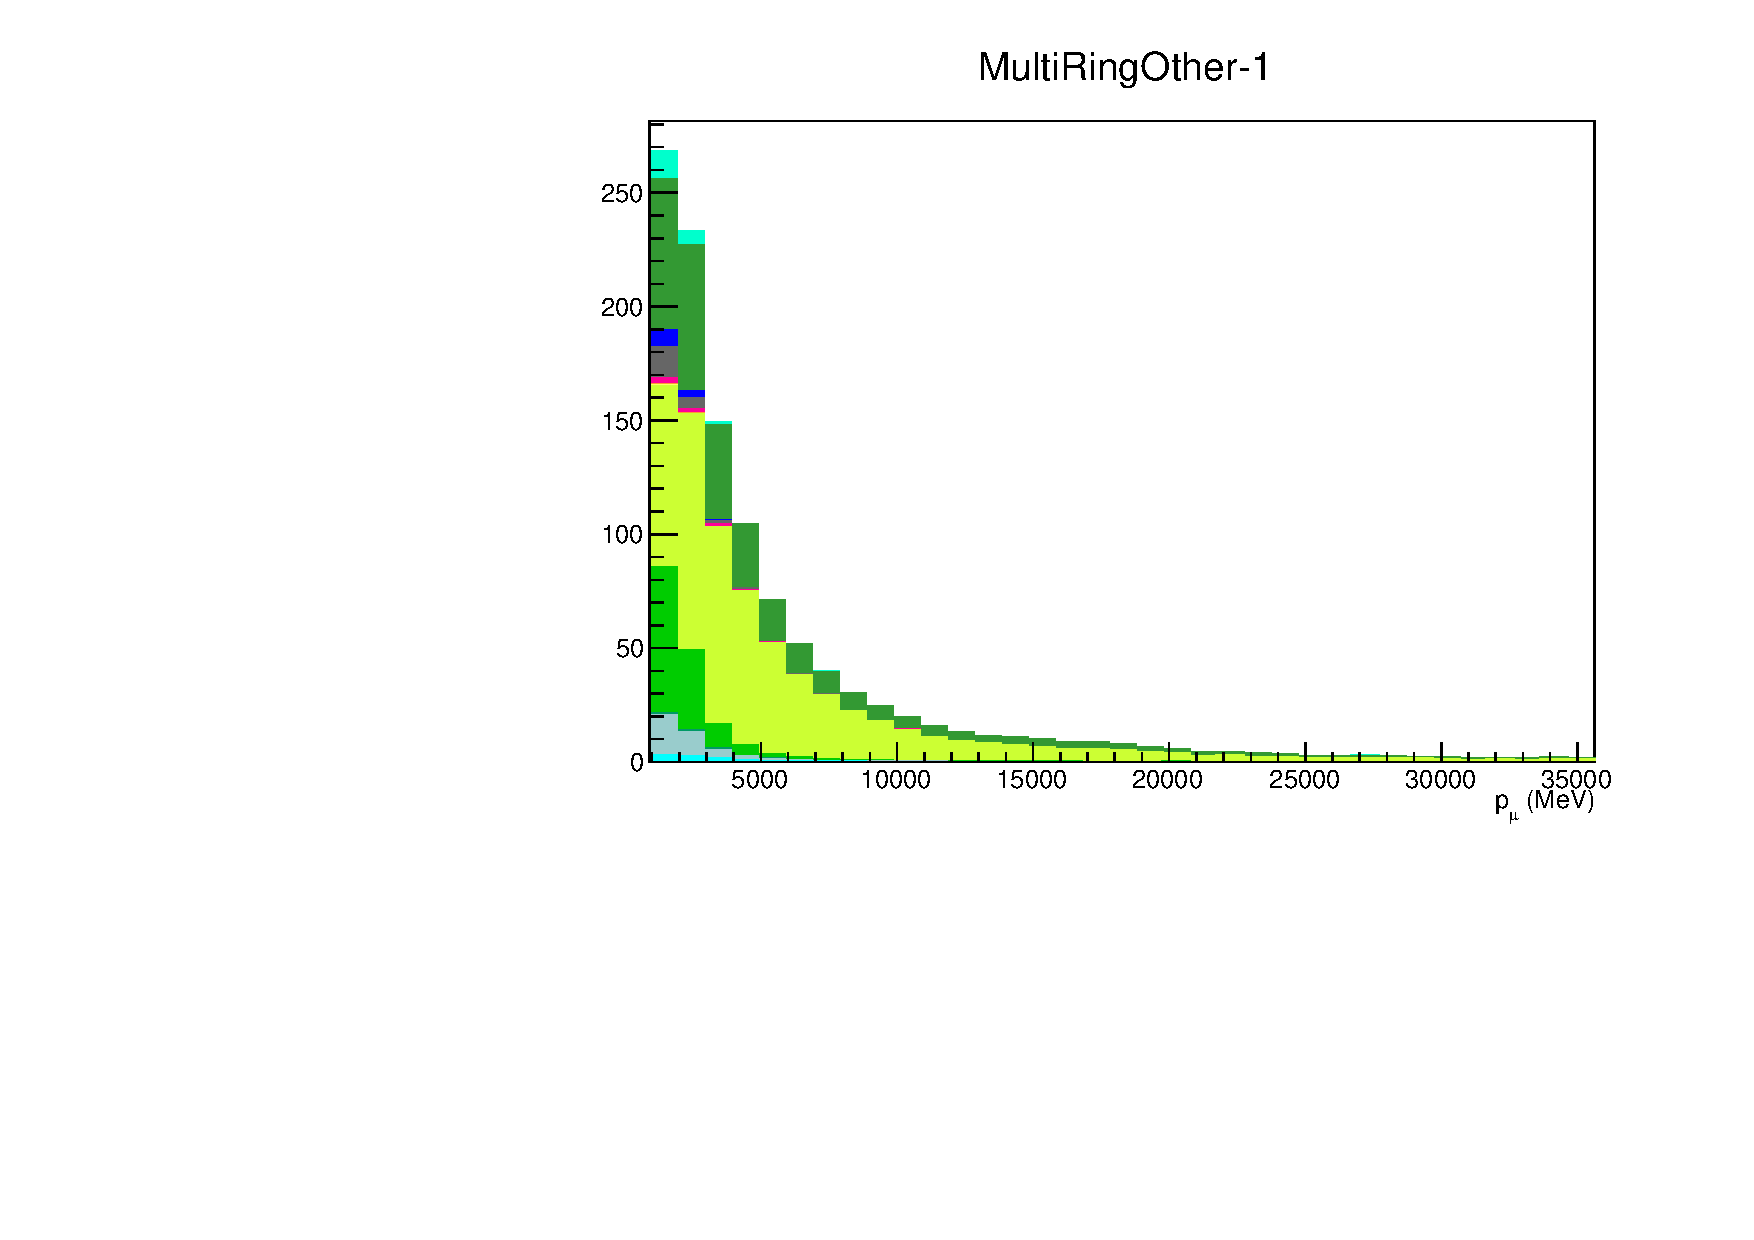
\includegraphics[width=\textwidth, trim= 0 0 0 30, clip]{Figures/Selections/AtmosphericByMode/MultiRingOther-1_LepMom.pdf}
    \caption{FC Multi-GeV multi-ring Other}
    \end{subfigure}
    \begin{subfigure}[t]{0.49\textwidth}
      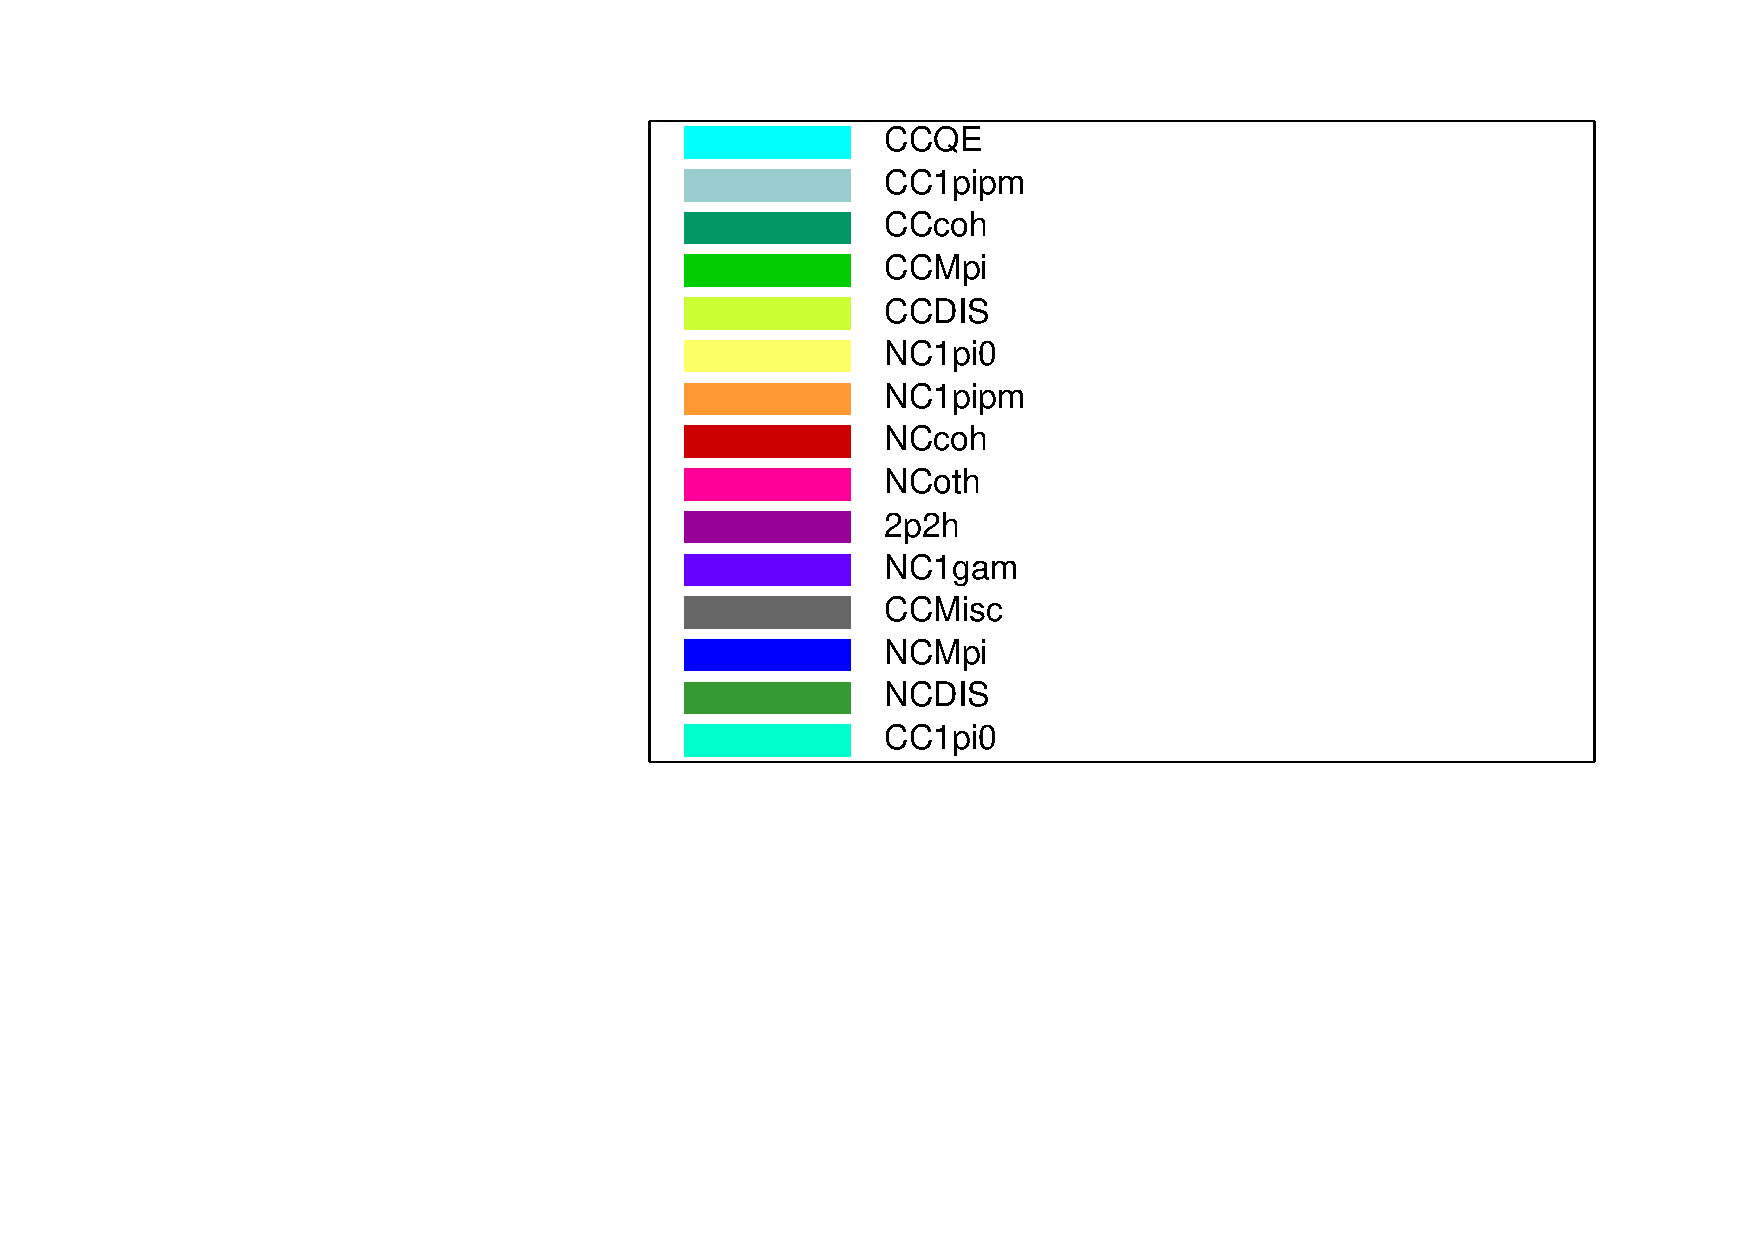
\includegraphics[page=1,width=\textwidth, trim= 0 0 0 30, clip]{Figures/Selections/AtmosphericByMode/Legend.pdf}
    \end{subfigure}
    
    \caption{Breakdown by interaction mode of the FC Multi-GeV  multi-ring atmospheric samples.}
    \label{fig:SKSamples:FCMultiRing}
\end{figure}

\clearpage
\section{Partially Contained Samples}
The breakdown for partially contained samples is highlighted in \autoref{fig:SKSamples:PC}. As with the multi-ring samples, there is no dominating interaction mode. The neutrino energies of events in this sample extend into the tens of GeV and become dominated by DIS interaction modes in the high energy limit.

\begin{figure}[ht]
    \begin{subfigure}[t]{0.49\textwidth}
    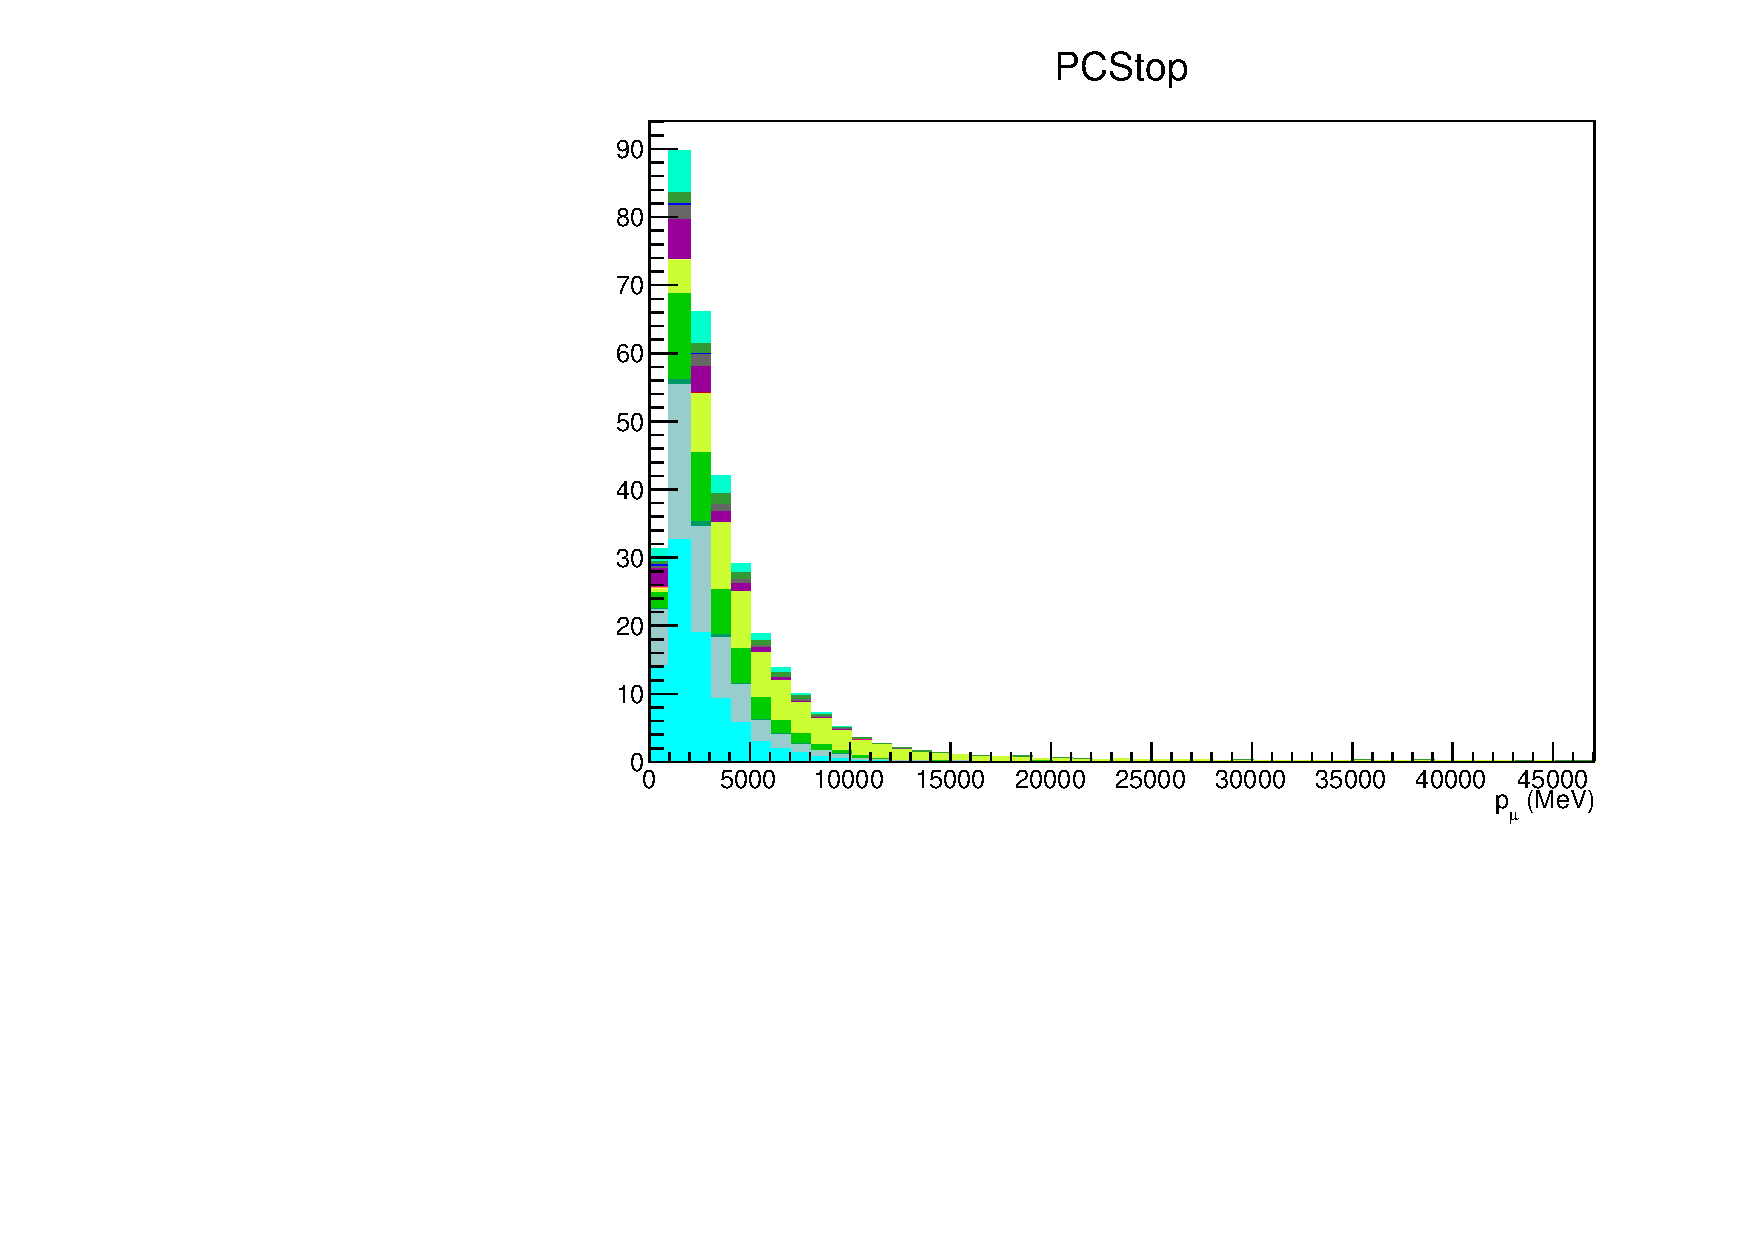
\includegraphics[width=\textwidth, trim= 0 0 0 30, clip]{Figures/Selections/AtmosphericByMode/PCStop_LepMom.pdf}
    \caption{PC stopping events}
    \end{subfigure}
    \begin{subfigure}[t]{0.49\textwidth}
    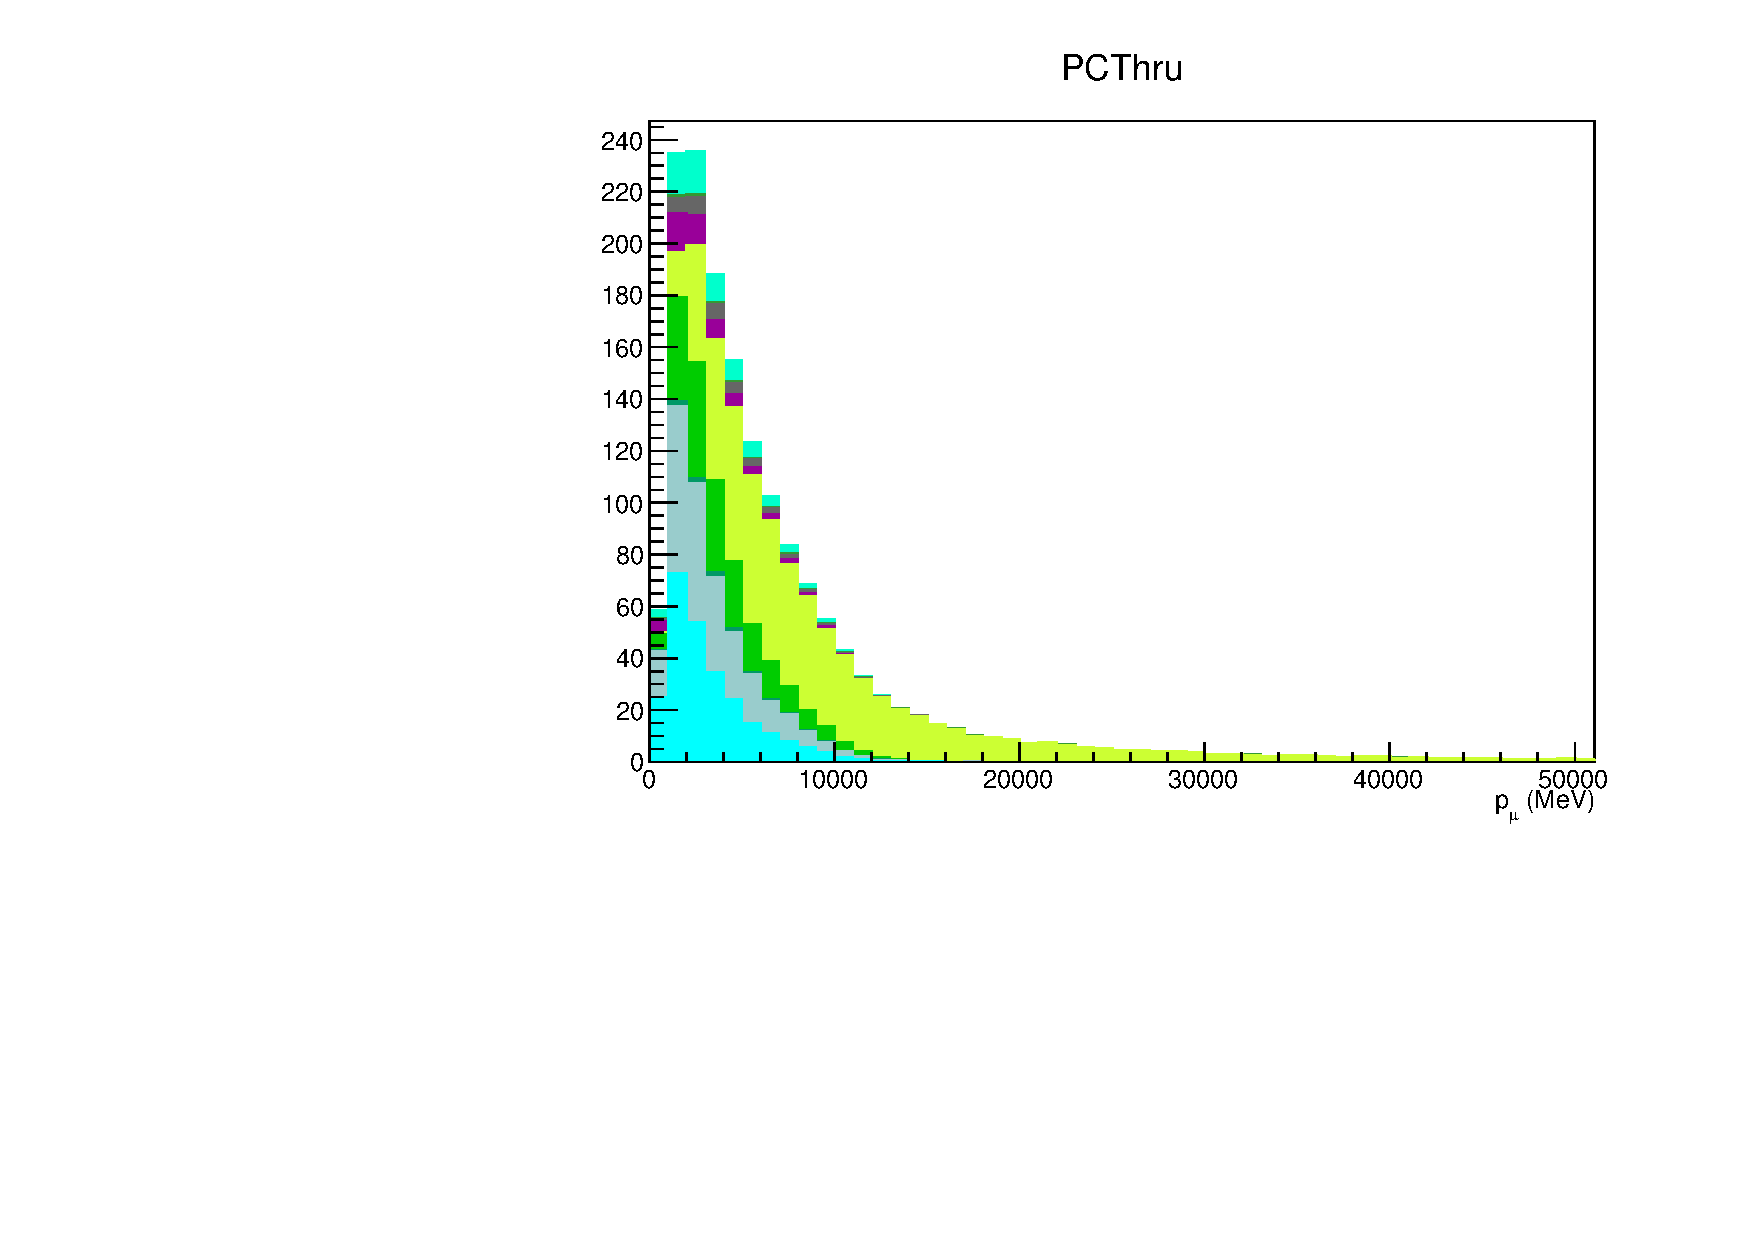
\includegraphics[width=\textwidth, trim= 0 0 0 30, clip]{Figures/Selections/AtmosphericByMode/PCThru_LepMom.pdf}
    \caption{PC through-going events.}
    \end{subfigure}
    \begin{subfigure}[t]{0.49\textwidth}
    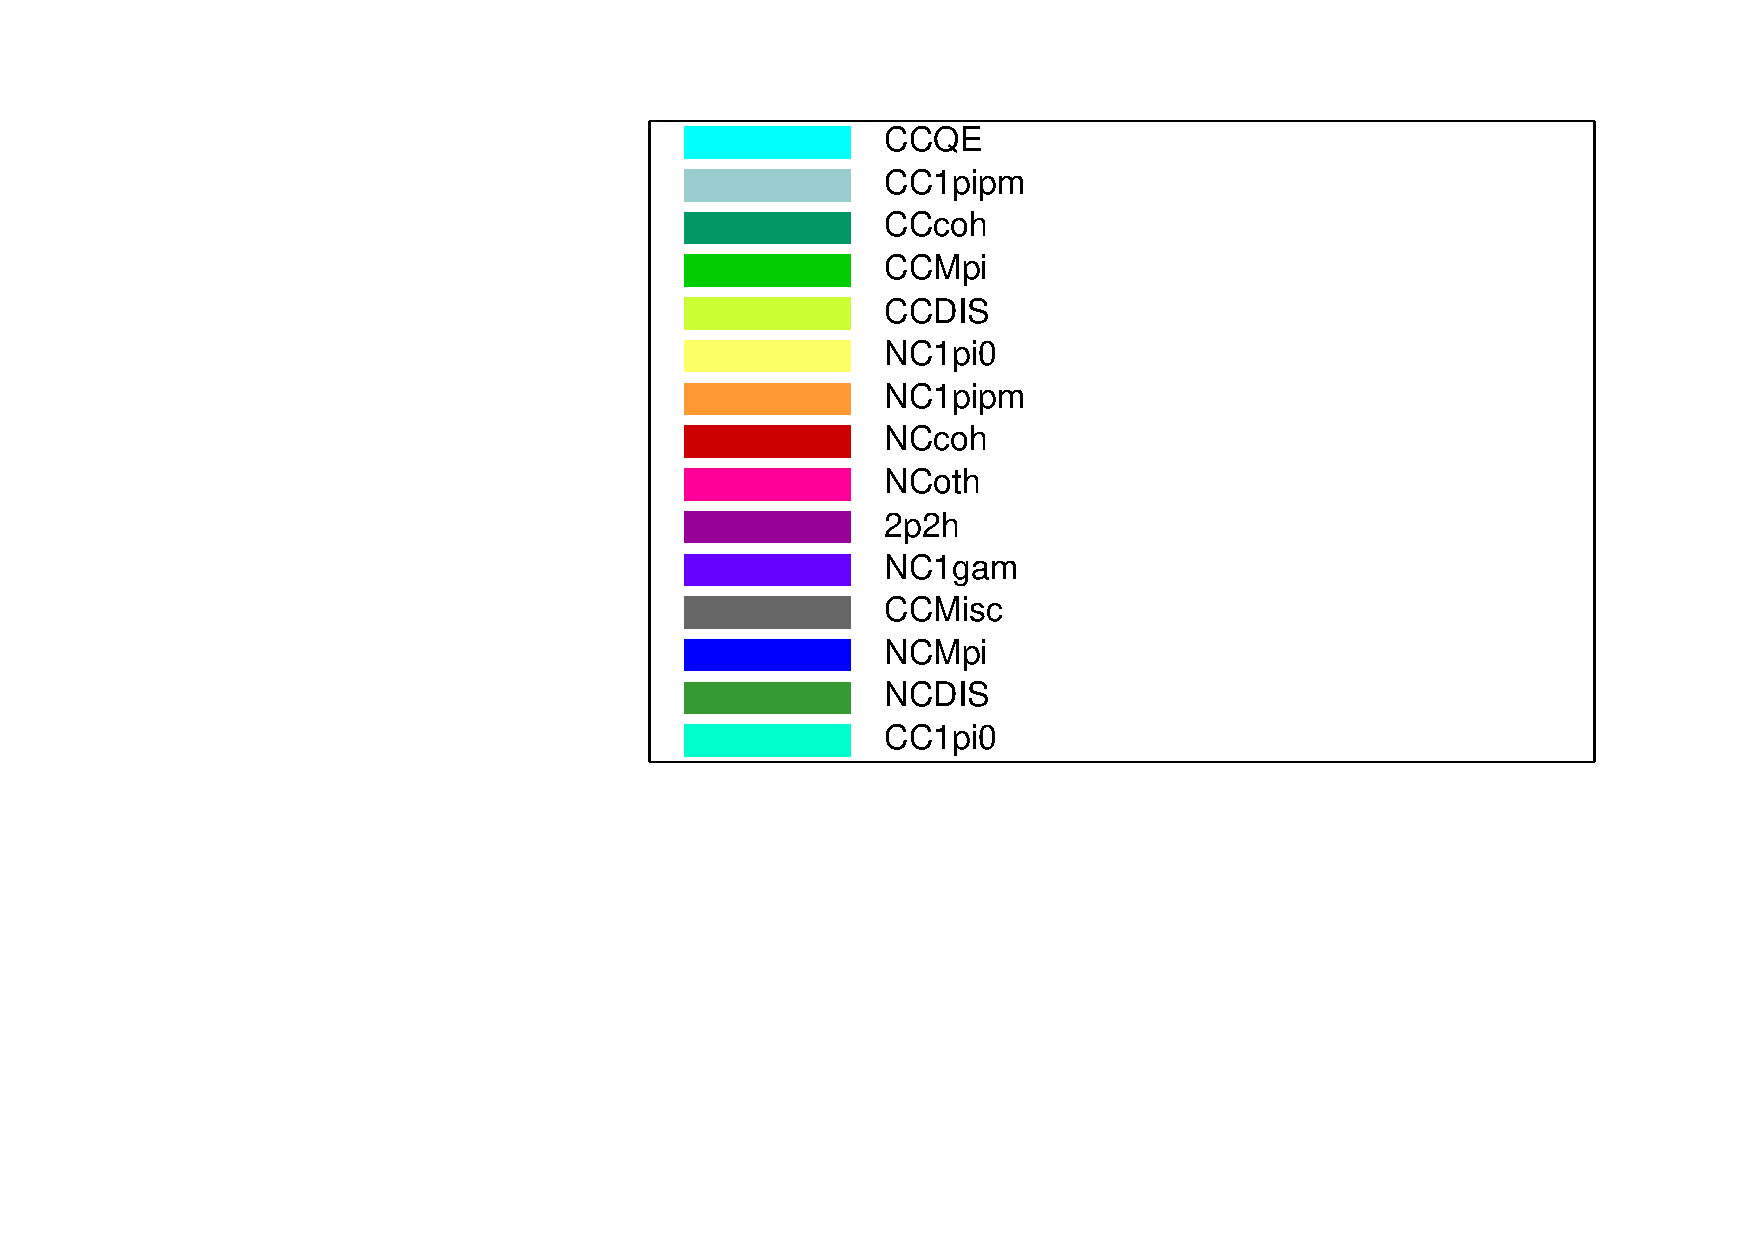
\includegraphics[page=1,width=\textwidth, trim= 0 0 0 30, clip]{Figures/Selections/AtmosphericByMode/Legend.pdf}
    \end{subfigure}
    
    \caption{Breakdown by interaction mode of the PC atmospheric samples.}
    \label{fig:SKSamples:PC}
\end{figure}

\clearpage
\section{Upward-Going Muon Samples}
The breakdown for upward-going muons is illustrated in \autoref{fig:SKSamples:Upmu}. These samples are significantly dominated by DIS interactions with energies extending up into the hundreds of GeV.

\begin{figure}[ht]
    \begin{subfigure}[t]{0.49\textwidth}
    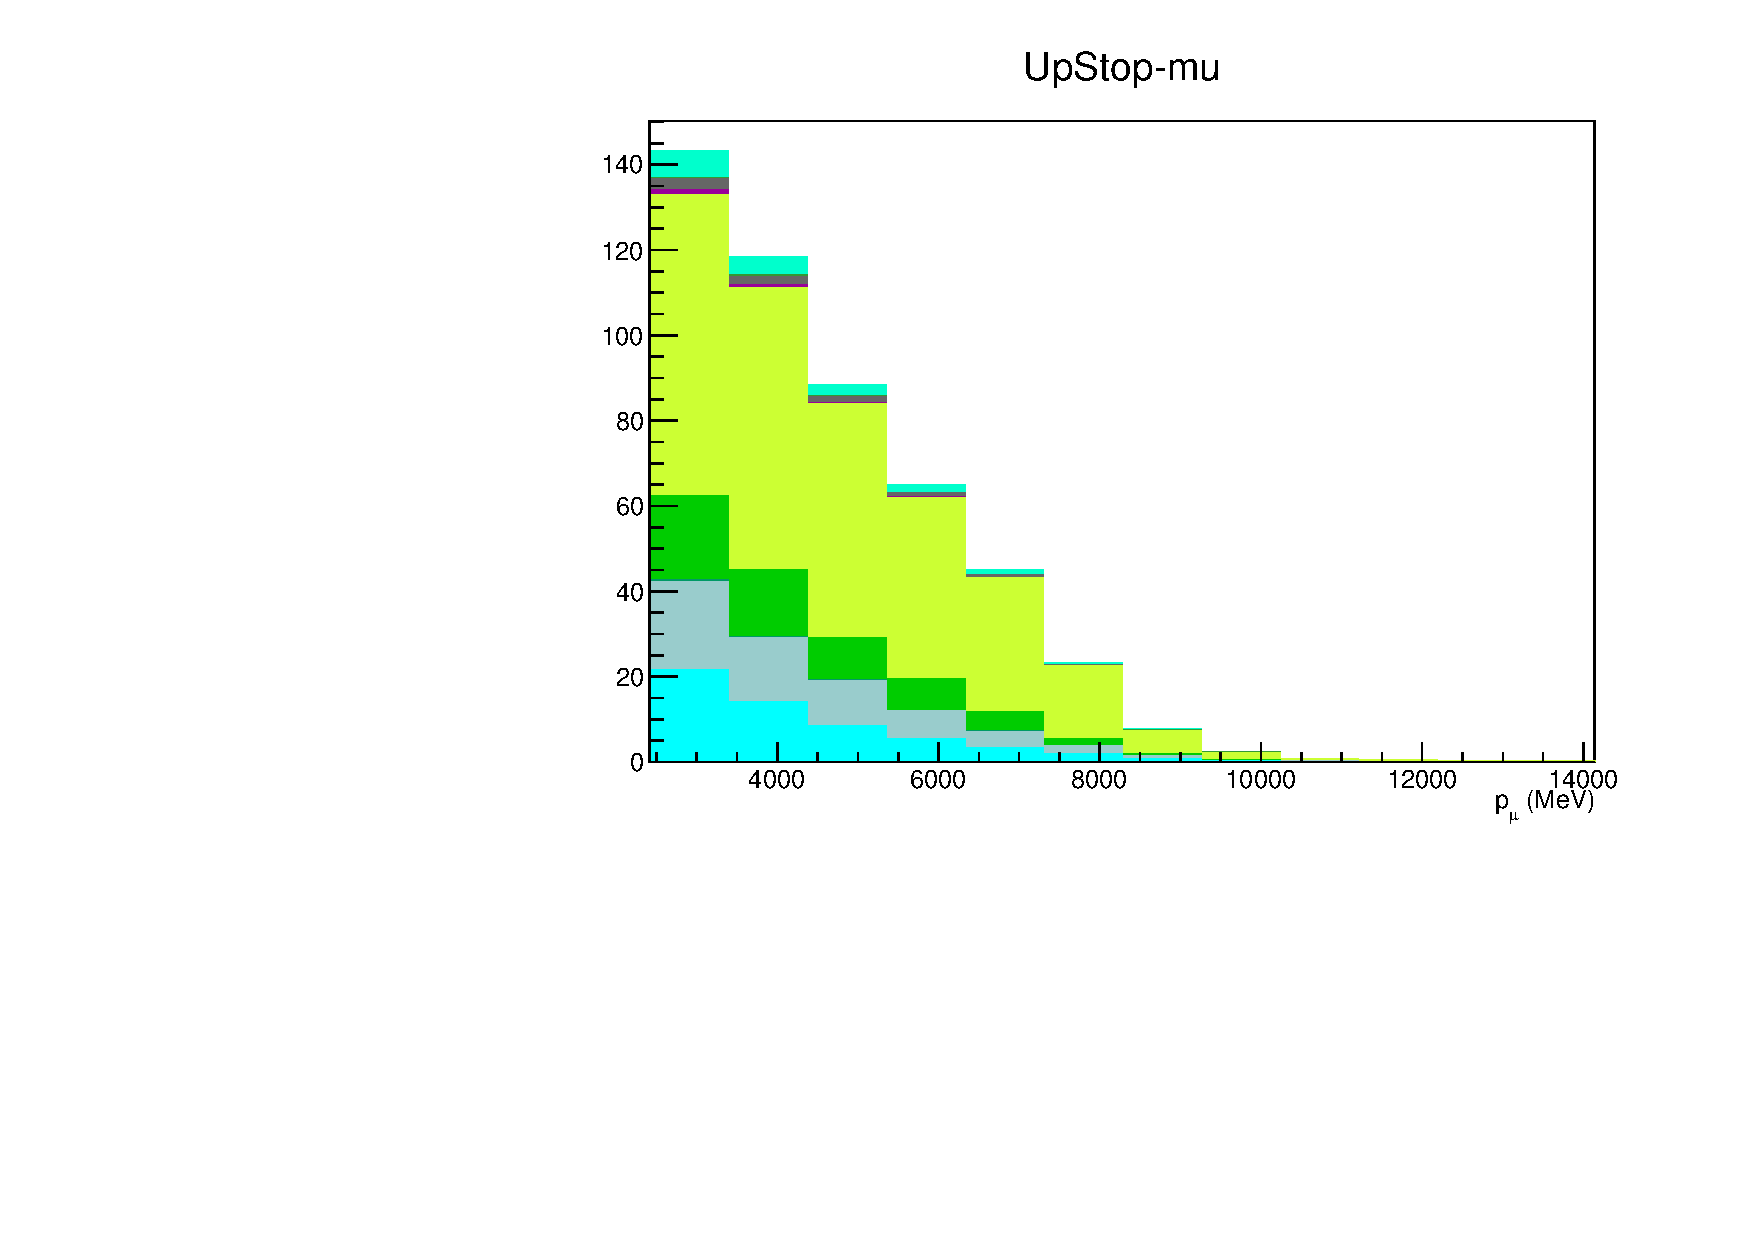
\includegraphics[width=\textwidth, trim= 0 0 0 30, clip]{Figures/Selections/AtmosphericByMode/UpStop-mu_LepMom.pdf}
    \caption{Up-$\mu$ stopping events}
    \end{subfigure}
    \begin{subfigure}[t]{0.49\textwidth}
    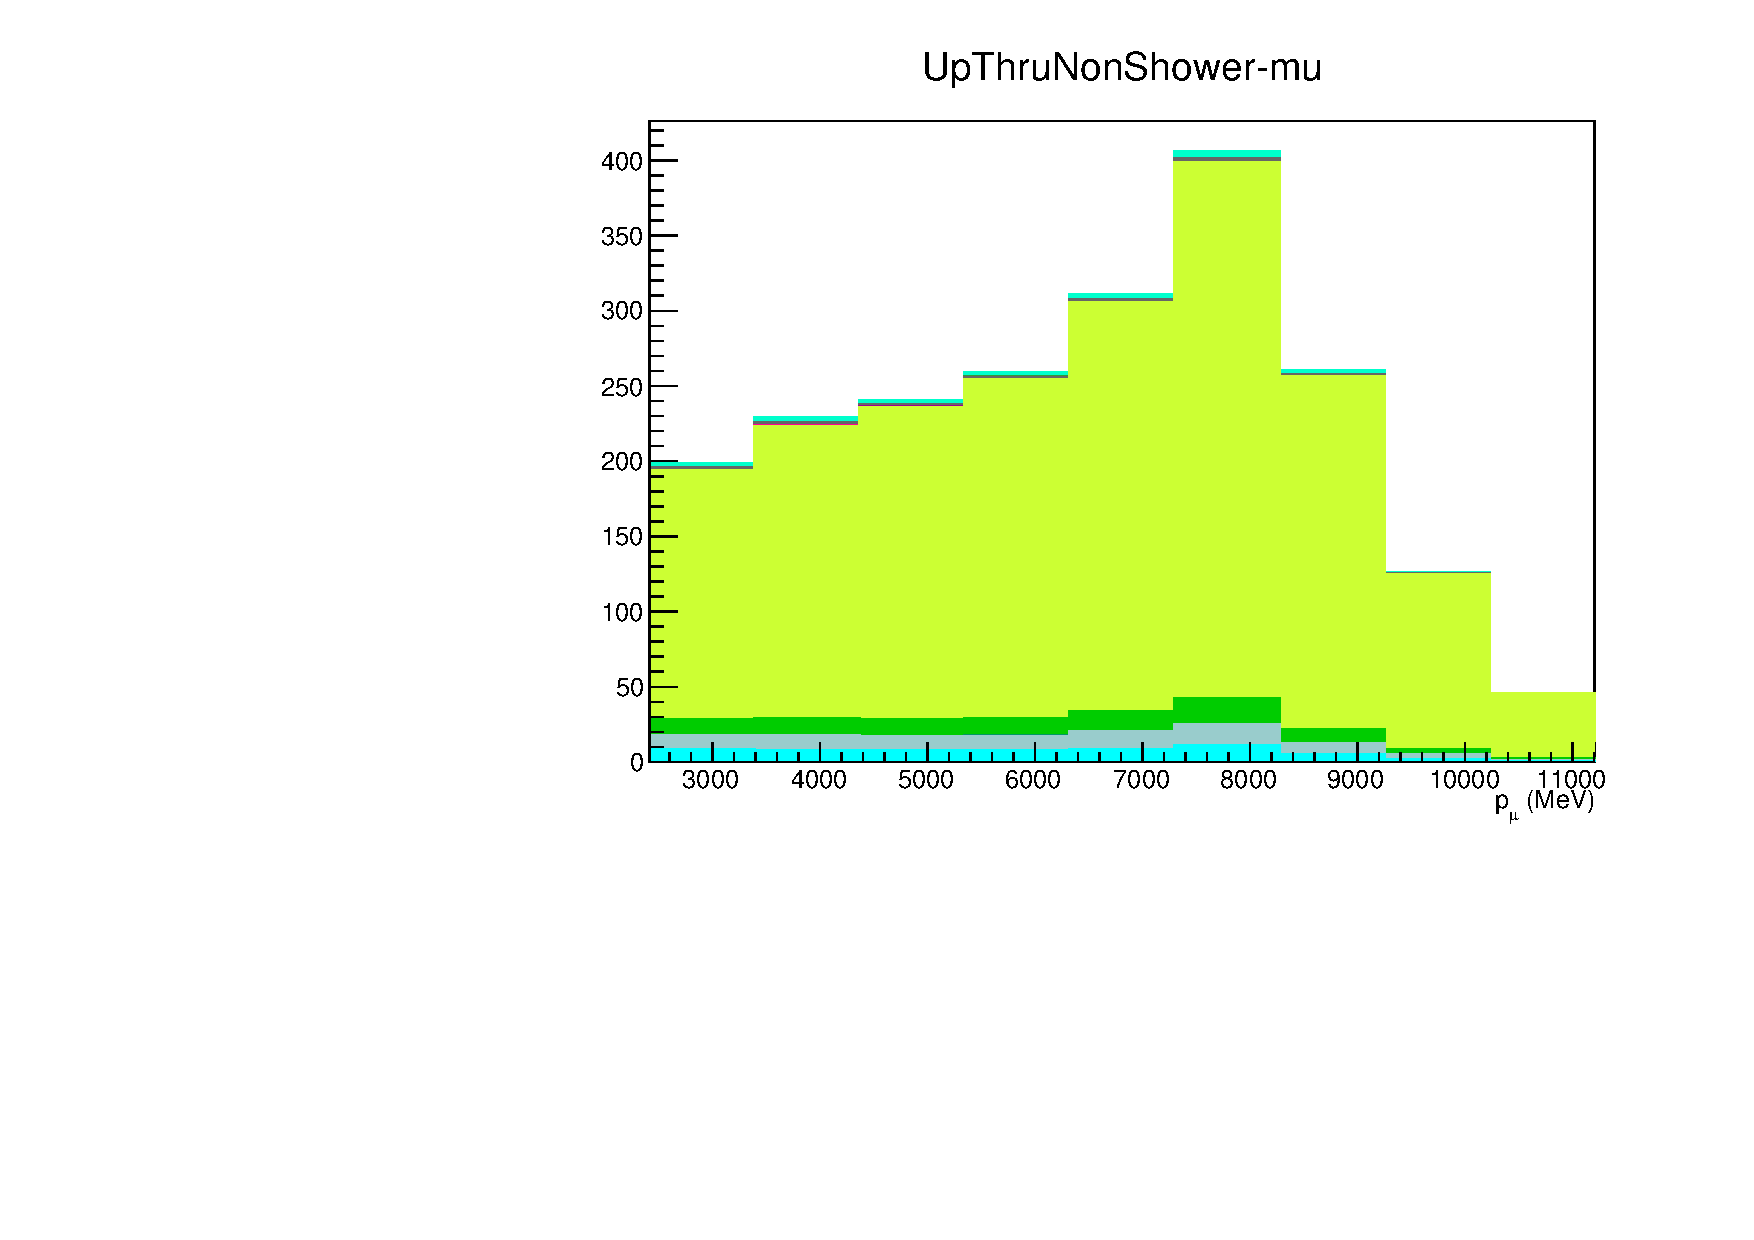
\includegraphics[width=\textwidth, trim= 0 0 0 30, clip]{Figures/Selections/AtmosphericByMode/UpThruNonShower-mu_LepMom.pdf}
    \caption{Up-$\mu$ through going non showering events}
    \end{subfigure}
    \begin{subfigure}[t]{0.49\textwidth}
    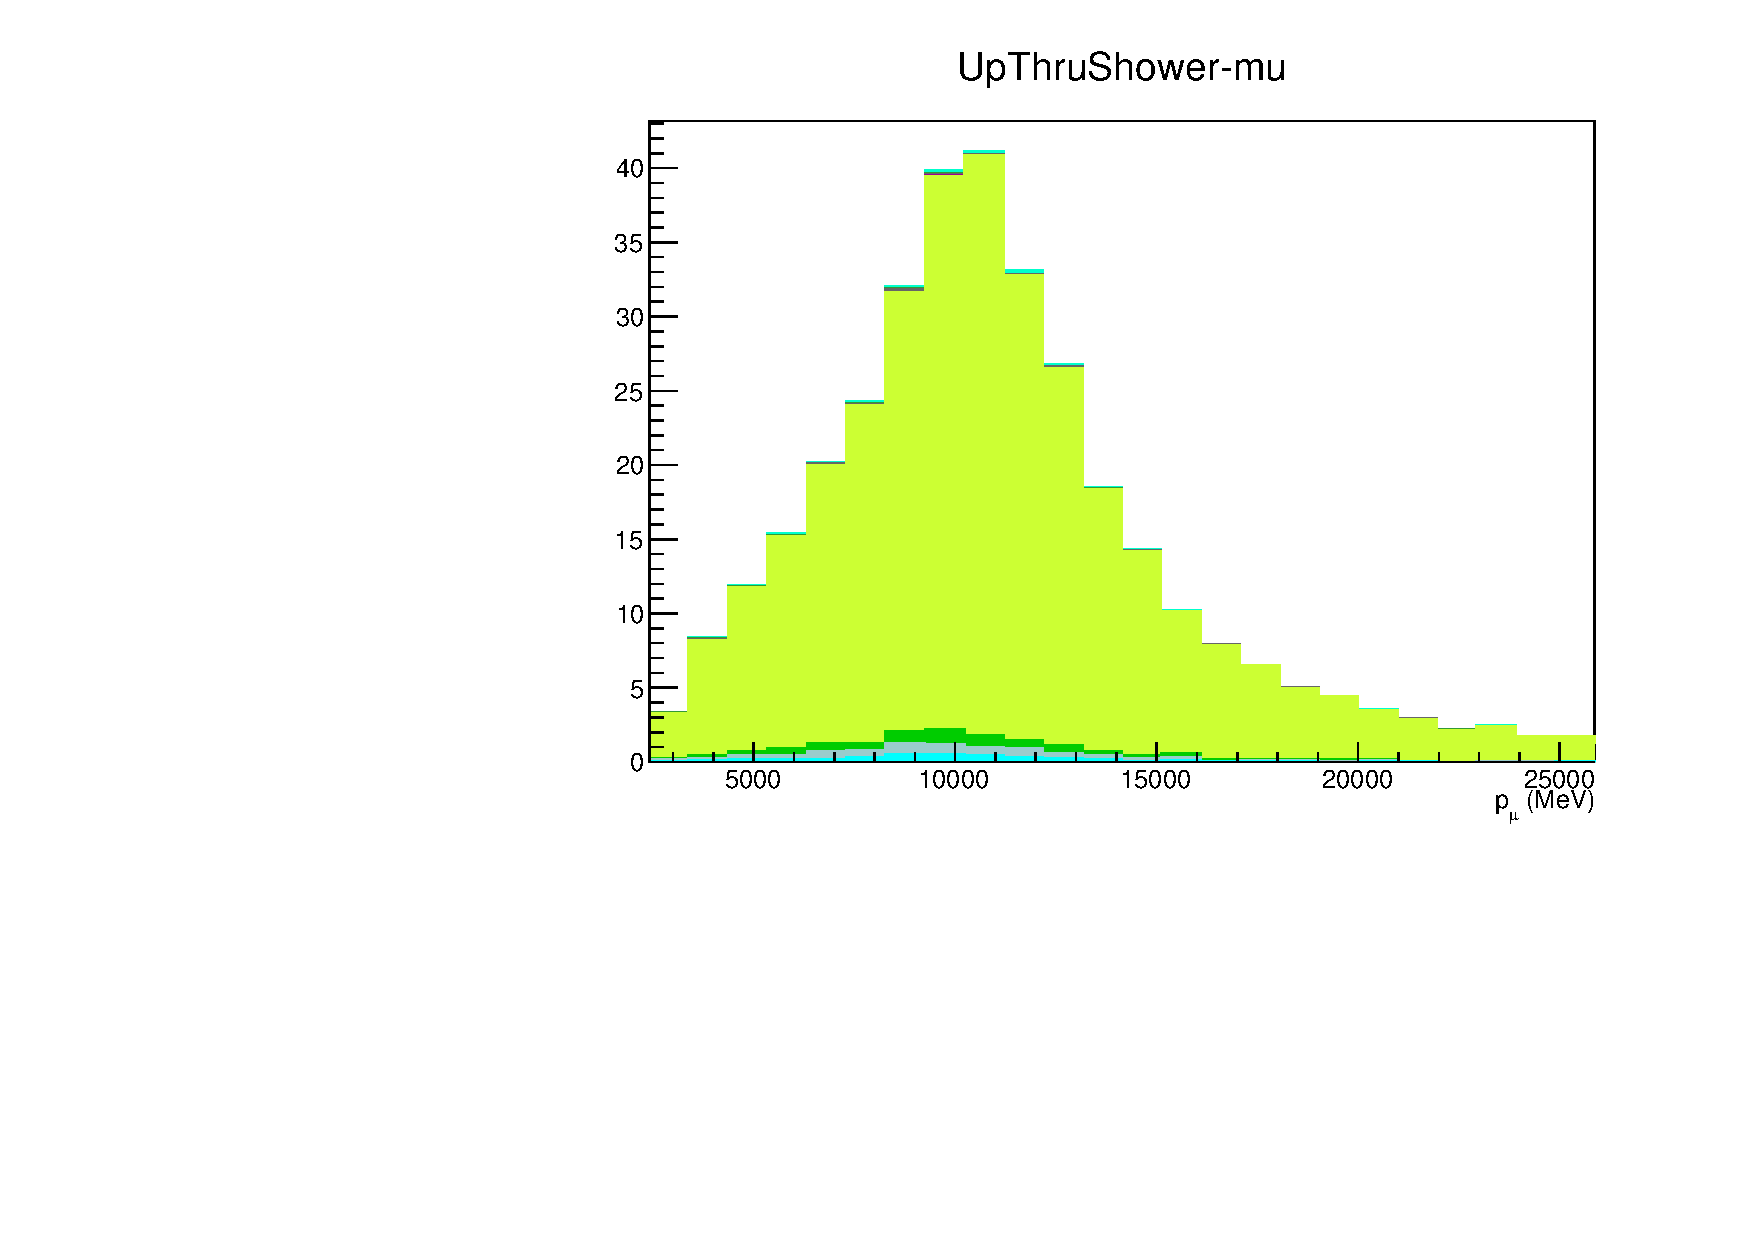
\includegraphics[width=\textwidth, trim= 0 0 0 30, clip]{Figures/Selections/AtmosphericByMode/UpThruShower-mu_LepMom.pdf}
    \caption{Up-$\mu$ through going showering events}
    \end{subfigure}
    \begin{subfigure}[t]{0.49\textwidth}
    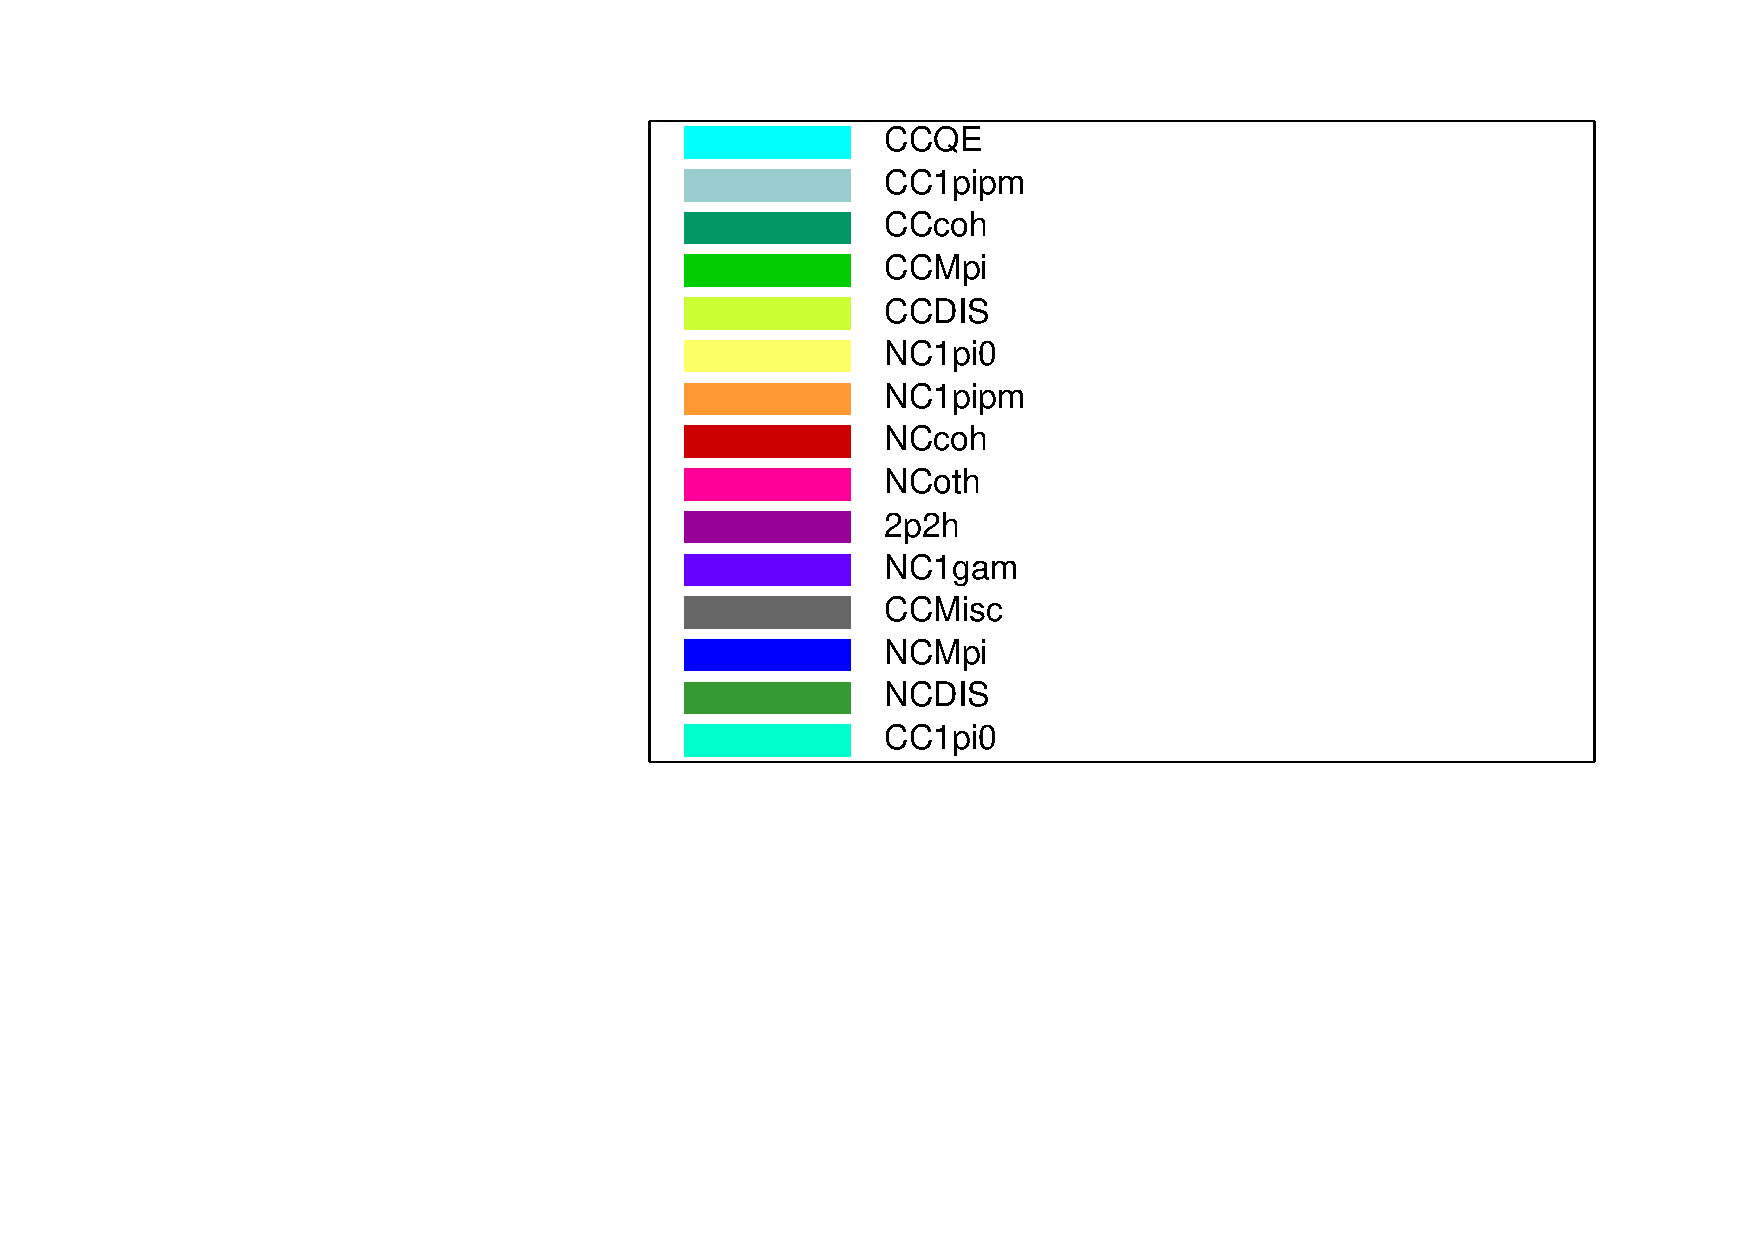
\includegraphics[width=\textwidth, page=1]{Figures/Selections/AtmosphericByMode/Legend.pdf}
    \end{subfigure}

    \caption{Breakdown by interaction mode of the atmospheric upward going muon samples.}
    \label{fig:SKSamples:Upmu}
\end{figure}
